\documentclass[10pt]{beamer}
\usepackage[utf8]{inputenc}

\usepackage{biblatex}
\bibliography{ref.bib}

\usetheme{Madrid}
\usecolortheme{default}
\useinnertheme{circles}

\definecolor{Logo1}{rgb}{0.208, 0.2865, 0.373}
\definecolor{Logo2}{rgb}{0.000, 0.674, 0.863}

\setbeamercolor*{palette primary}{bg=Logo1, fg=white}
\setbeamercolor*{palette secondary}{bg=Logo2, fg=white}
\setbeamercolor*{palette tertiary}{bg=white, fg=Logo1}
\setbeamercolor*{palette quaternary}{bg=Logo1,fg=white}
\setbeamercolor{structure}{fg=Logo1} % itemize, enumerate, etc
\setbeamercolor{section in toc}{fg=Logo1} % TOC sections

%------------------------------------------------------------
%This block of code defines the information to appear in the
%Title page
\title[Object States Estimation] %optional
{Object Classification, Detection and State Estimation using YOLO-v3 Deep Neural
Network and Sensor Fusion of Stereo Camera and LiDAR}

\author[K. Mehta] % (optional)
{Kamalkumar Mehta\\
 Supervisor: Dr. Kamesh Subbarao}

\institute[UTA] % (optional)
{
  Aerospace System Laboratory\\
  Department of Mechanical and Aerospace Engineering\\
  The University of Texas at Arlington
}

\logo{
\includegraphics[width=0.05\textwidth]{UTA.png}} 
 

\date % (optional)
{Master Dissertation, June 2021}

%End of title page configuration block
%------------------------------------------------------------



%------------------------------------------------------------
%The next block of commands puts the table of contents at the 
%beginning of each section and highlights the current section:

\AtBeginSection[]
{
  \begin{frame}
    \frametitle{Table of Contents}
    \tableofcontents[currentsection]
  \end{frame}
}
%------------------------------------------------------------


\begin{document}

%The next statement creates the title page.
\frame{\titlepage}

%---------------------------------------------------------
%This block of code is for the table of contents after
%the title page
\begin{frame}
\frametitle{Table of Contents}
\tableofcontents
\end{frame}
%---------------------------------------------------------

%%%%%%%%%%%%%%%% Starts From Here %%%%%%%%%%%%%%%%%%%%%%%%


%%%%%%% Motivation & Background %%%%%%%%
\section{Motivation \& Background}

%---------------------------------------------------------
%Changing visibility of the text
\begin{frame}
\frametitle{Motivation}
\begin{itemize}
    \item Real-time object detection framework plays essential part in an autonomous drivers assistance system (ADAS) to avoid collision with other vehicles. 
    \item It has wide use in many autonomous tasks such collision avoidance in self-driving vehicle, simultaneous localization and mapping (SLAM) in a mobile robot, personal security, surveillance, target tracking, and identity verification.   
    \item The other object detection frameworks have few drawbacks which limits the use in real-time object detection application.  
    \item Whereas, YOLO is the unified approach to objects detection which requires \alert{single regression training} and have \alert{faster inference time}.   
\end{itemize}
\end{frame}

\begin{frame}
\frametitle{Background}
\begin{itemize}
    \item The region proposal based object detection framework (R-CNN) was introduced by Girshick et al. in 2014 which integrates AlexNet and region based selective search. \footnote[frame]{\fullcite{girshick2014}}
    \item To overcome the drawbacks of R-CNN, improved versions Fast-RCNN and Faster-RCNN has been proposed by Girshick et al. in 2015 and Ren et al. in 2016 respectively. \footnote[frame]{\fullcite{ren2016faster}}
    \item Redmon et al. in 2016 introduced the unified object detection framework (YOLO) that passes the input image once to detect objects. \footnote[frame]{\fullcite{redmon2016}}
    \item Further improvement done by Redmon and Farhadi and proposed YOLO-v3 in 2018 in order to increase accuracy in detection. \footnote[frame]{\fullcite{yolov3}}   
\end{itemize}

\end{frame}

\begin{frame}
\frametitle{Data Pipeline}
\centering
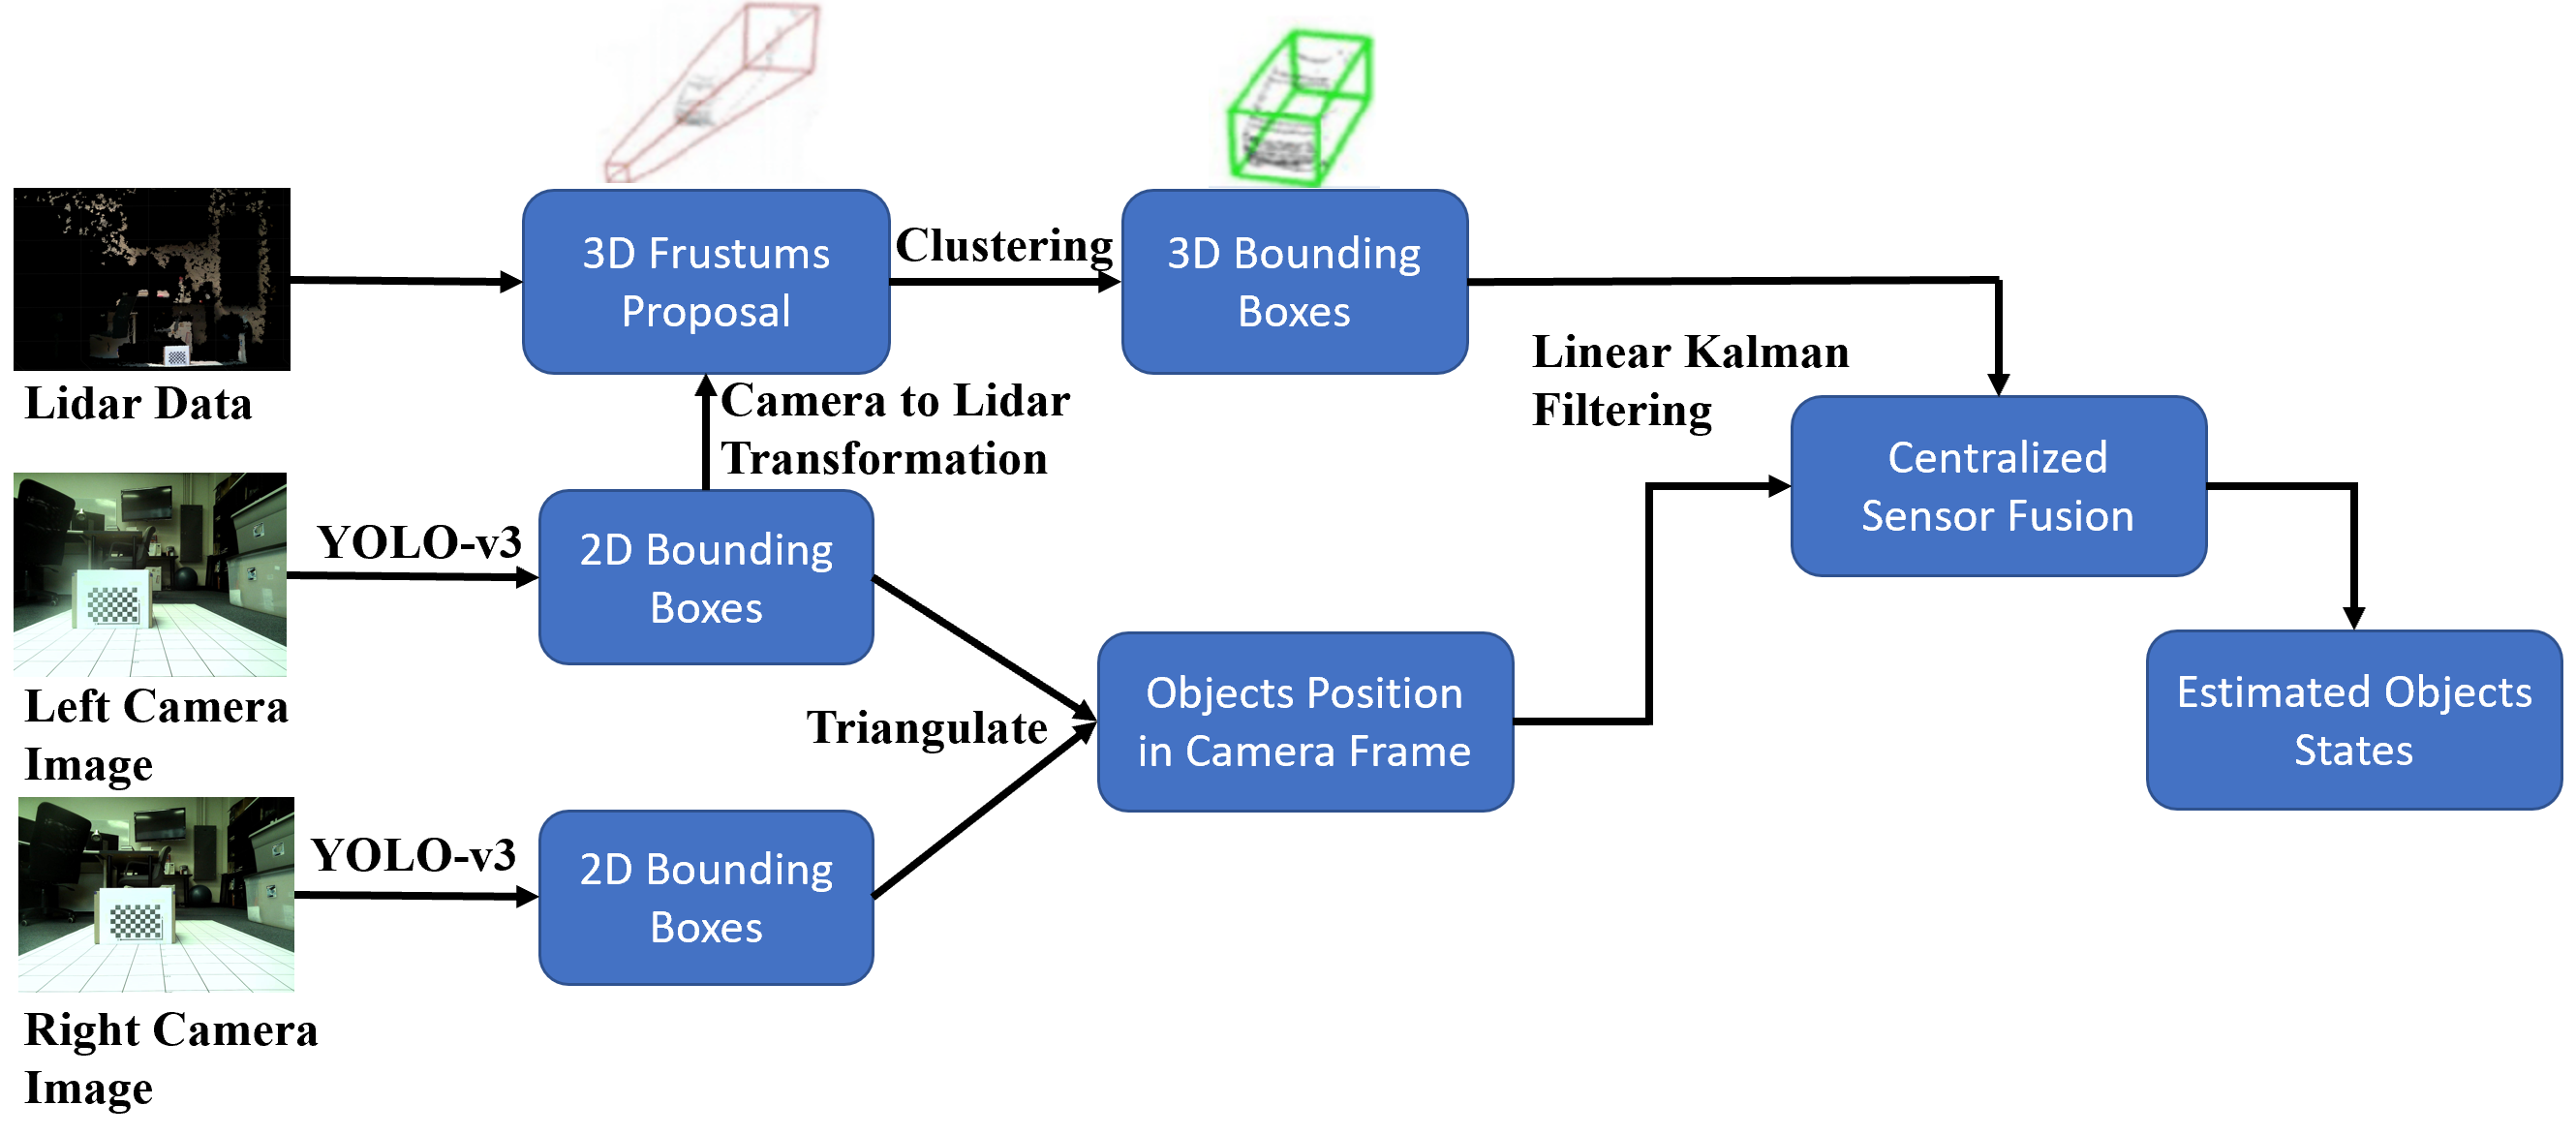
\includegraphics[width = 1\textwidth]{Images/Datapipeline.png}
\end{frame}
%---------------------------------------------------------

%%%%%%%YOLO-v3 Architecture%%%%%%%%

\section{YOLO-v3 Architecture}

%---------------------------------------------------------
%Highlighting text
\begin{frame}
\frametitle{YOLO-v3 Architecture}

\begin{figure}
    \centering
    \fbox{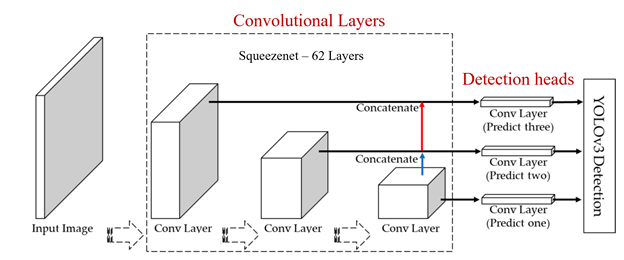
\includegraphics[width=0.9\textwidth,height=2in]{Images/layersYOLO.png}}
    \caption{Stacks of Layers in YOLO-v3 Network \footnote[frame]{\fullcite{rs12010044}}}
\end{figure}

\end{frame}

\begin{frame}{Layers in Neural Network Architecture}
    \begin{columns}
       \column{0.45\textwidth}
        \begin{block}{Input Layer}
         \begin{itemize}
             \item Filters the Input Image which size does not compatible to network
         \end{itemize}             
        \end{block}
        \vspace{-5pt}
        \begin{block}{Convolutional Layer}
         \begin{itemize}
             \item Performs convolutional operation to detects features from the image e.g. edges, textures, patterns, and parts
             \item Convolutional operation reduces the size of input image 
             \item The size of filter is pre-define based on the level of feature needs to detect
             \item Each filter learns one feature of the image
         \end{itemize}
        \end{block}

        \column{0.45\textwidth}
        \begin{block}{Non-linear Activation Layer}
            \begin{itemize}
               \item Impose low-level non-linearity in feature map generated by Conv. layer.
               \item Reduce the bias in overall training error. 
            \end{itemize} 
        \end{block} 
        
        \begin{example}{Non-linear Activation}
             \begin{figure}
                  \centering
                   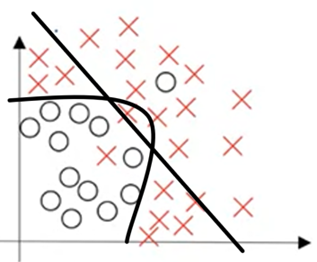
\includegraphics[width=0.6\textwidth]{Images/activation.png}
            \end{figure}
        \end{example}
    \end{columns}
\end{frame}

\begin{frame}{Layers in Neural Network Architecture}
    \begin{columns}
       \column{0.5\textwidth}
        \begin{block}{Pooling or Down-sampling Layer}
         \begin{itemize}
             \item Extracts the most significant number from image by pre-defined size of window
             \item Reduce computational load, increase speed in training, and prevent over-fitting
         \end{itemize}             
        \end{block}
        \vspace{-5pt}
        \begin{block}{Fully Connected Layer}
         \begin{itemize}
             \item To combine all the features detected by the Conv. layer and generate classification score for each class
             \item All the nodes of fully-connected layer are connected with each element of the Conv. layer
             \item Because of too many connections, learning process slows down 
         \end{itemize}
        \end{block}

        \column{0.4\textwidth}
        \begin{block}{Up-sampling Layer}
             \begin{itemize}
                \item Recover the original Image by increase the resolution of activation 
                \item ''Skip-connection" is efficient way to recover the high-resolution of image
                \item Mainly use in task when high resolution is essential e.g. object localization \& detection
                \item Slows down the processing time 
            \end{itemize}
        \end{block} 
    \end{columns}
\end{frame}

%---------------------------------------------------------

%%%%%%%Supervised Learning%%%%%%%%

\section{Supervised Learning}

%---------------------------------------------------------

\begin{frame}{Data Preprocessing}
    \begin{figure}
        \centering
        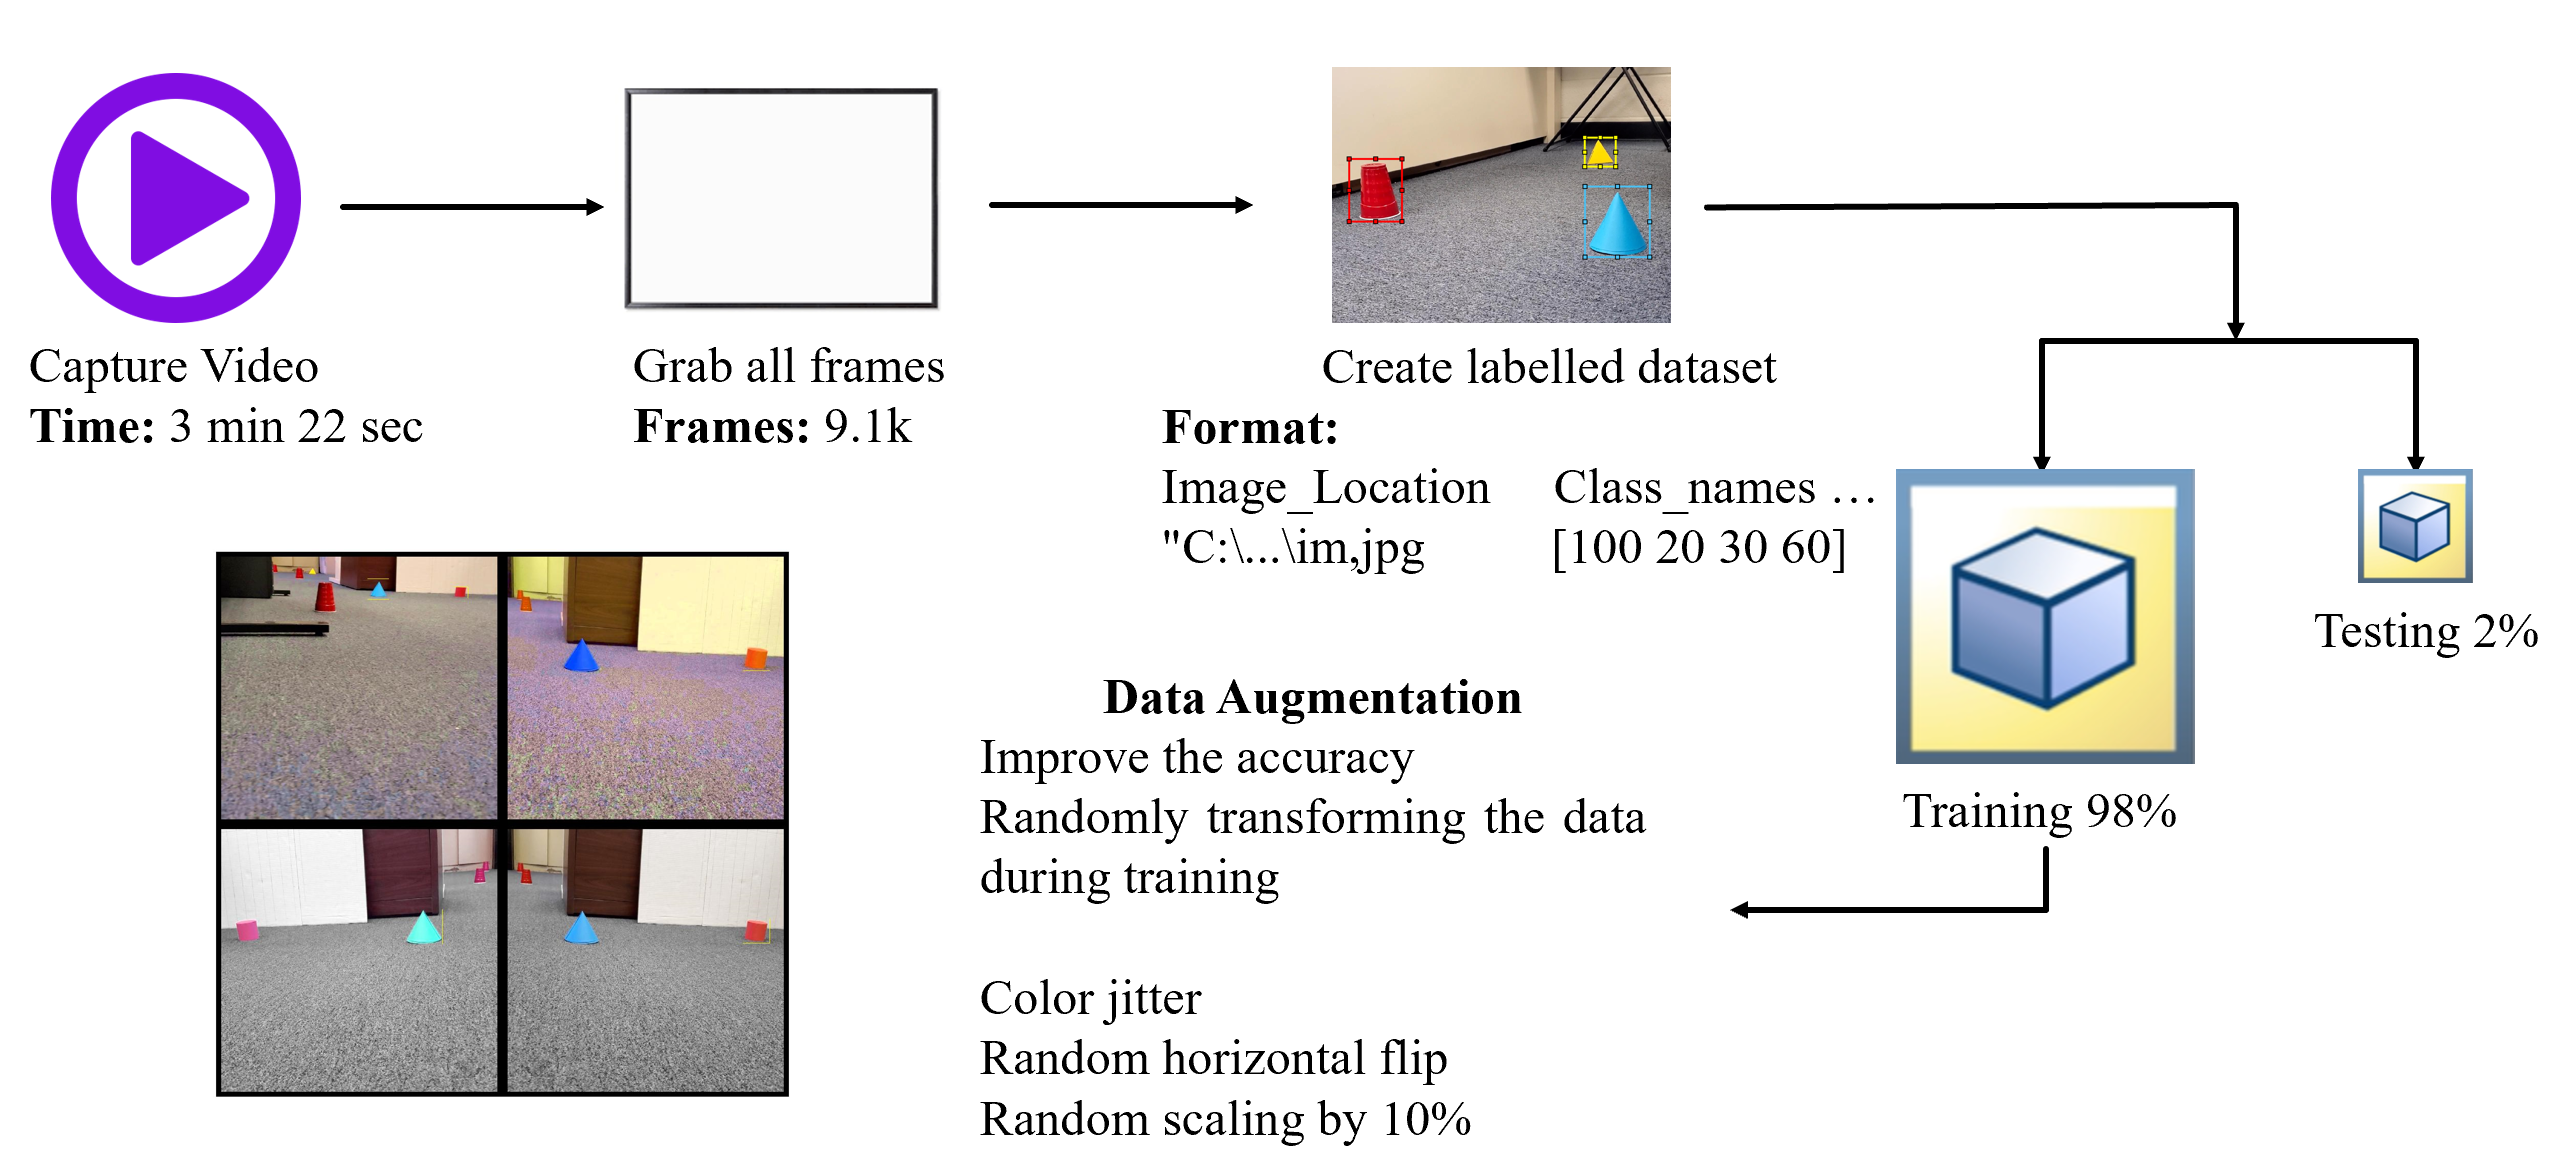
\includegraphics[width=1\textwidth]{Images/datapreprocess.png}
    \end{figure}  
\end{frame}

\begin{frame}{Stochastic Gradient Descent with Momentum (SGDM)}
   \begin{itemize}
       \item Neural network impose has non-linearity that causes the most of the loss function to become non-convex
       \item Iterative gradient descent based optimization of appropriate convex function with proper parameter initialization leads to the global minima. 
   \end{itemize}
   
\begin{block}{Loss Function}
     \begin{columns}
            \column{0.5\textwidth}
            \begin{figure}
                \centering
                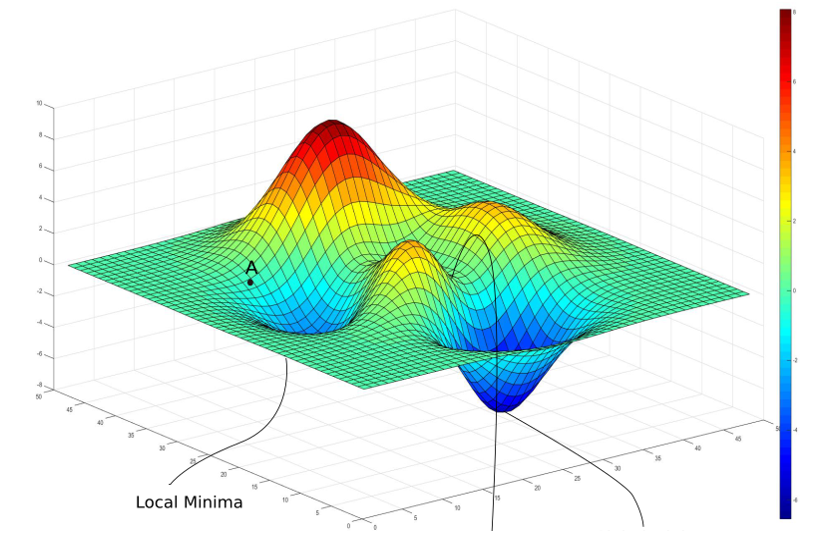
\includegraphics[width=0.5\textwidth]{Images/nonconvex.png}
                \caption{Non-convex \footnote[frame]{\fullcite{Convexity}}}
            \end{figure}
            \vspace{-5pt}
            \centering
            $\mathcal{L}(\hat{y}, y)=\frac{1}{2}(\hat{y}-y)^{2}$
            
            \column{0.5\textwidth}
            \begin{figure}
                \centering
                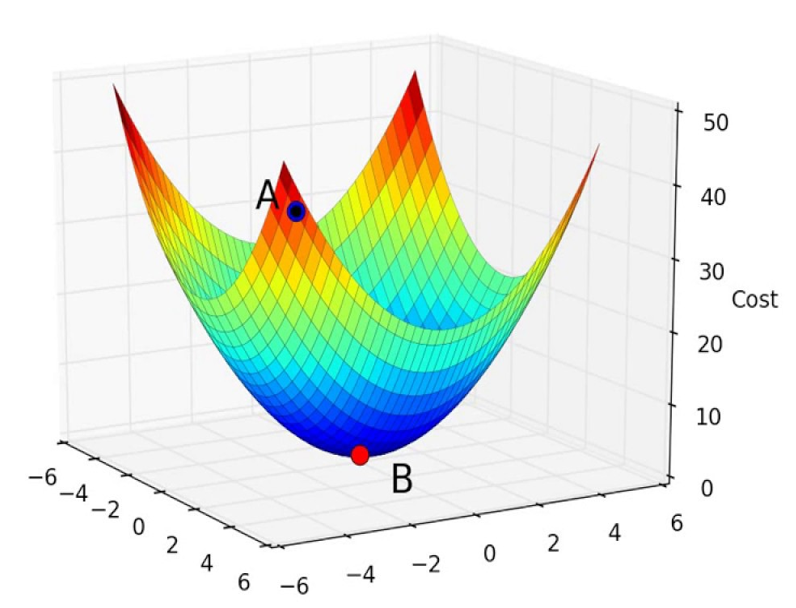
\includegraphics[width=0.5\textwidth]{Images/convex.png}
                \caption{Convex \footnote[frame]{\fullcite{Convexity}}}
            \end{figure}    
            \vspace{-5pt}
            \centering
            $\mathcal{L}(\hat{y}, y)=-(y \log \hat{y}+(1-y) \log (1-\hat{y}))$
     \end{columns}
\end{block}
\end{frame}

\begin{frame}{Stochastic Gradient Descent with Momentum (SGDM)}
    \begin{block}{Cost Function}
        \begin{itemize}
            \item Loss function is define for one training example, the extension of loss function for multiple training example is called cost function 
        \end{itemize}
            \vspace{1pt}
            \centering
            $$\mathcal{J}(\omega, b)=\frac{1}{m} \sum_{i=1}^{m} L\left(\hat{y}^{(i)}, y^{(i)}\right)=-\frac{1}{m} \sum_{i=1}^{m} [y^{(i)} \log \hat{y}^{(i)}+\left(1-y^{(i)}\right) \log \left(1 - \hat{y}^{(i)})\right]$$ 
    \end{block}
    
    \begin{block}{Momentum}
         \begin{itemize}
             \item SGDM is combination of the conventional gradient descent algorithm uses with momentum term 
             \item Momentum is defined by exponentially weighted average of training parameters as follows
         \end{itemize}
            \centering
            $V_{d W}=\beta v_{d W}+(1-\beta) d W$ \\
            $V_{d b}=\beta v_{d b}+(1-\beta) d b$
    \end{block}
\end{frame}

\begin{frame}{Stochastic Gradient Descent with Momentum (SGDM)}
    \begin{block}{Parameter updates}
         \begin{itemize}
             \item The momentum parameter $\beta$ represents how quick the gradient needs to move towards global minima and it should be between 0 and 1 
             \item Initial Bias correction: $\frac{V_{d W}}{1 - \beta^t}$
             \item Momentum term damping out the oscillations by averaging the positive and negative values in vertical direction 
             \item The training parameters updates after calculating momentum:  
         \end{itemize}
         \centering
         $W=W-\alpha \cdot V_{d W}$ \\
         $b=b-\alpha \cdot V_{d b}$  
         
        \begin{figure}
            \centering
            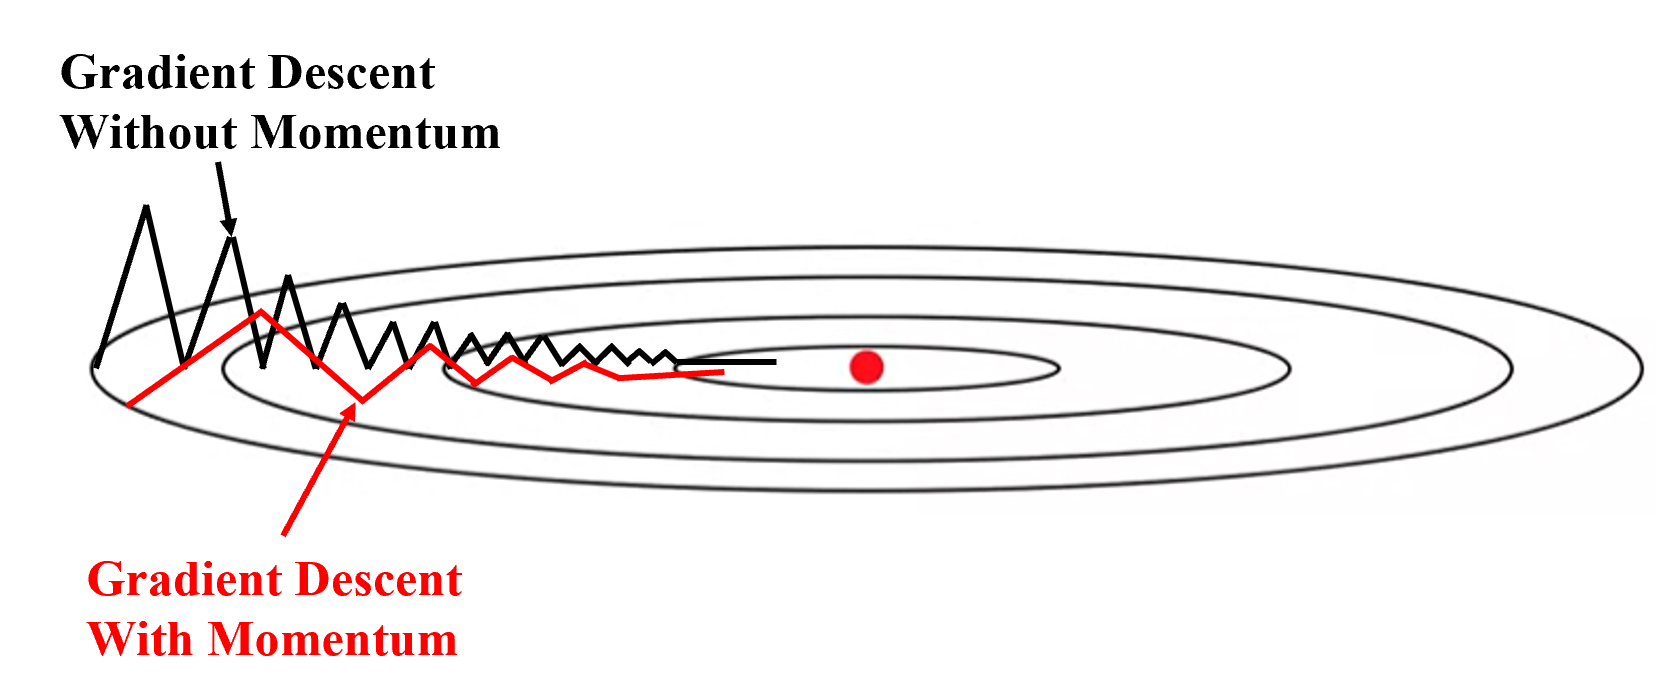
\includegraphics[width=0.45\textwidth]{Images/SGDM.png}
            \caption{Robustness of Stochastic Gradient Descent with Momentum}
        \end{figure}   
    \end{block}
\end{frame}

\begin{frame}{Stochastic Gradient Descent with Momentum (SGDM)}
    \begin{block}{Forward and Backward Propagation}
        \begin{itemize}
            \item \textbf{Backward Propagation:} Fine tune the training parameters based on the error from previous iteration
            \item \textbf{Forward Propagation:} Derive the amount of error after tuning of the training parameters 
        \end{itemize}
        \vspace{-5pt}
        \begin{figure}
             \centering
             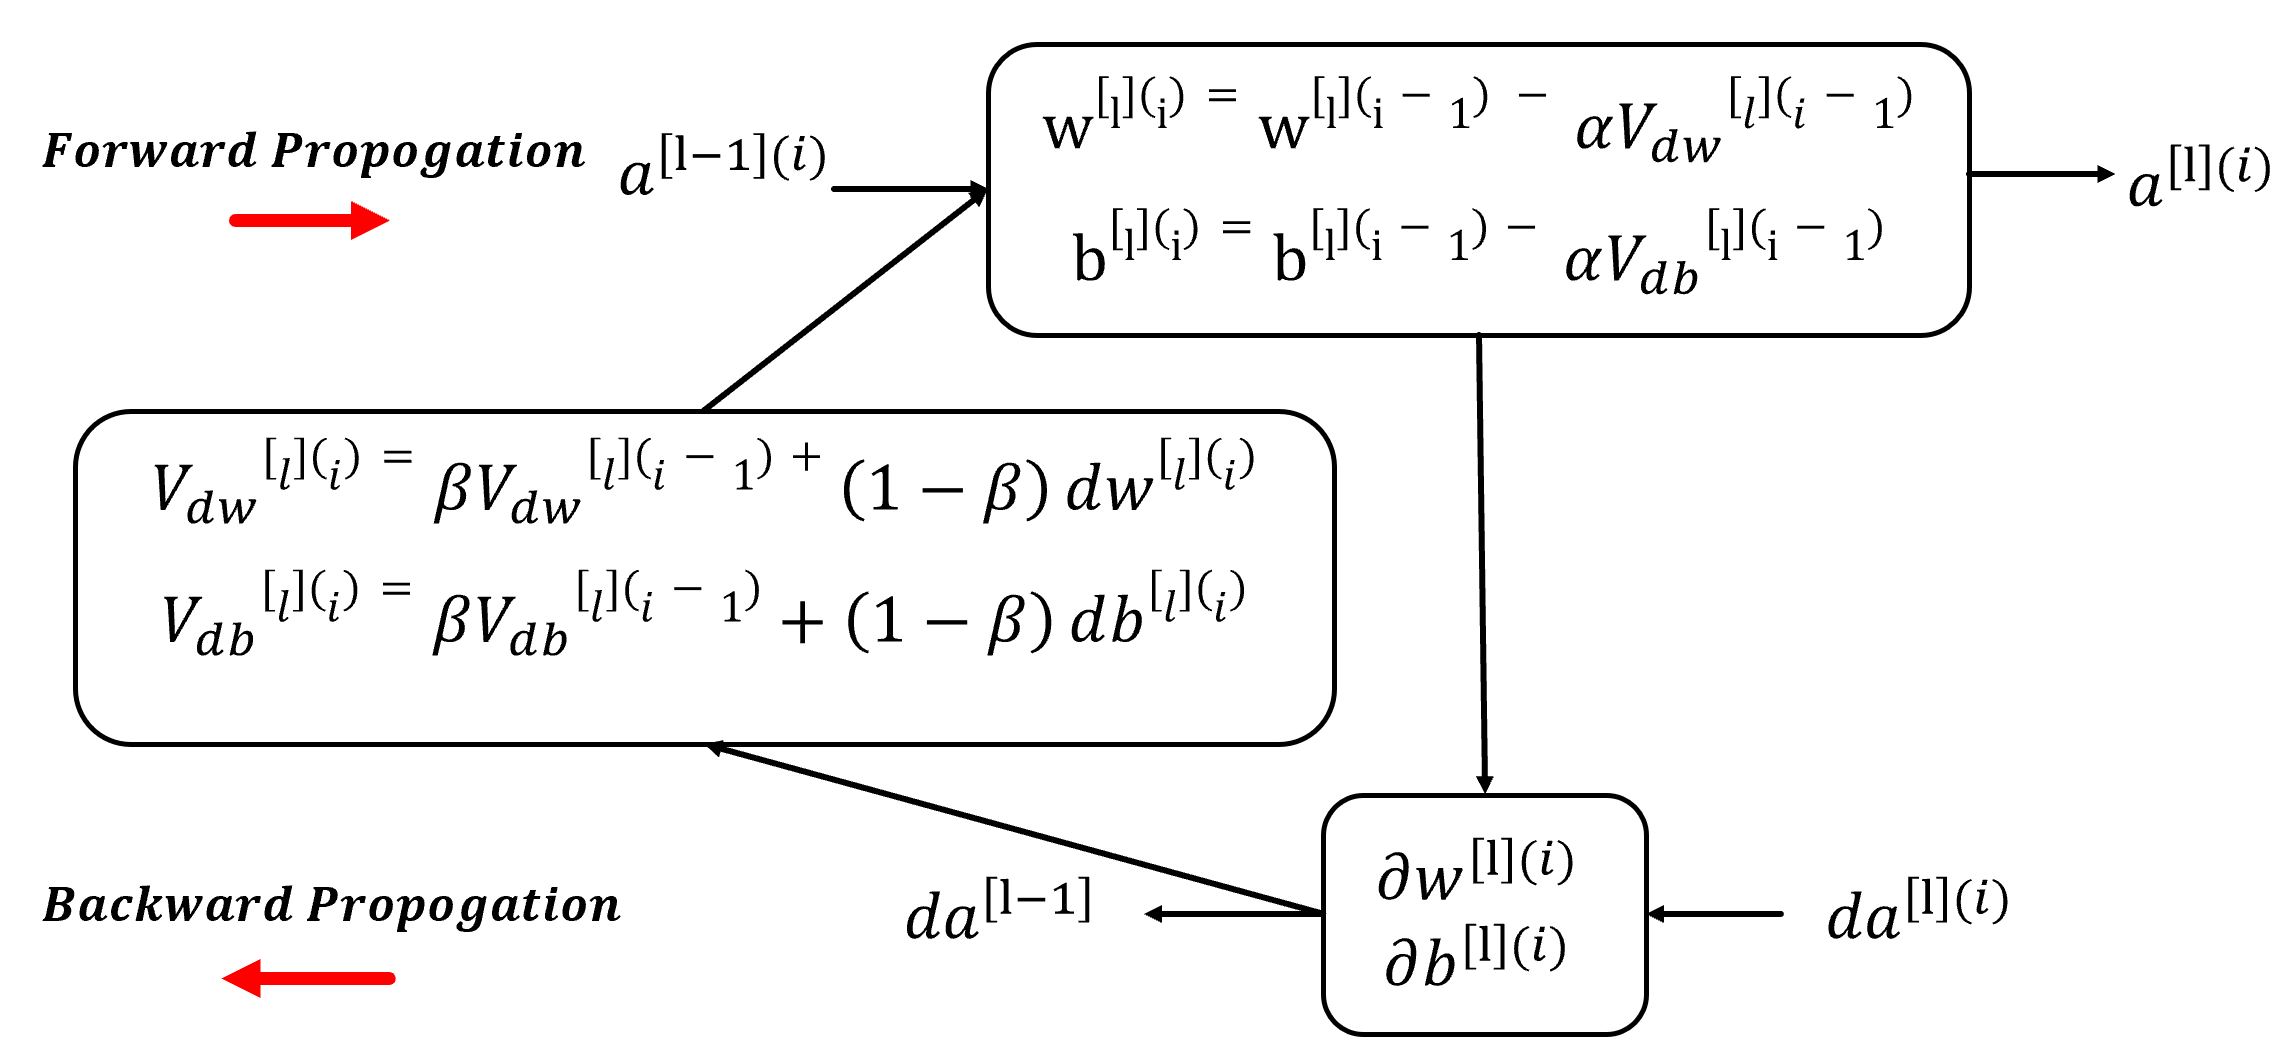
\includegraphics[width=0.9\textwidth]{Images/propogation.png}
        \end{figure} 
    \end{block}
\end{frame}

%---------------------------------------------------------

%%%%%%%Hyper-parameters Tuning%%%%%%%%

\section{Hyper-parameters Tuning}

%---------------------------------------------------------
\begin{frame}{Bias - Variance Trade-off}
   \begin{itemize}
       \item \textbf{Bias:} Error due to deviation in estimation from true value
       \item \textbf{Variance:} Error due to deviation in measurement from expectation
       \item Bias and Variance are inversely proportional to each other 
   \end{itemize}
   
   \begin{figure}
        \centering
        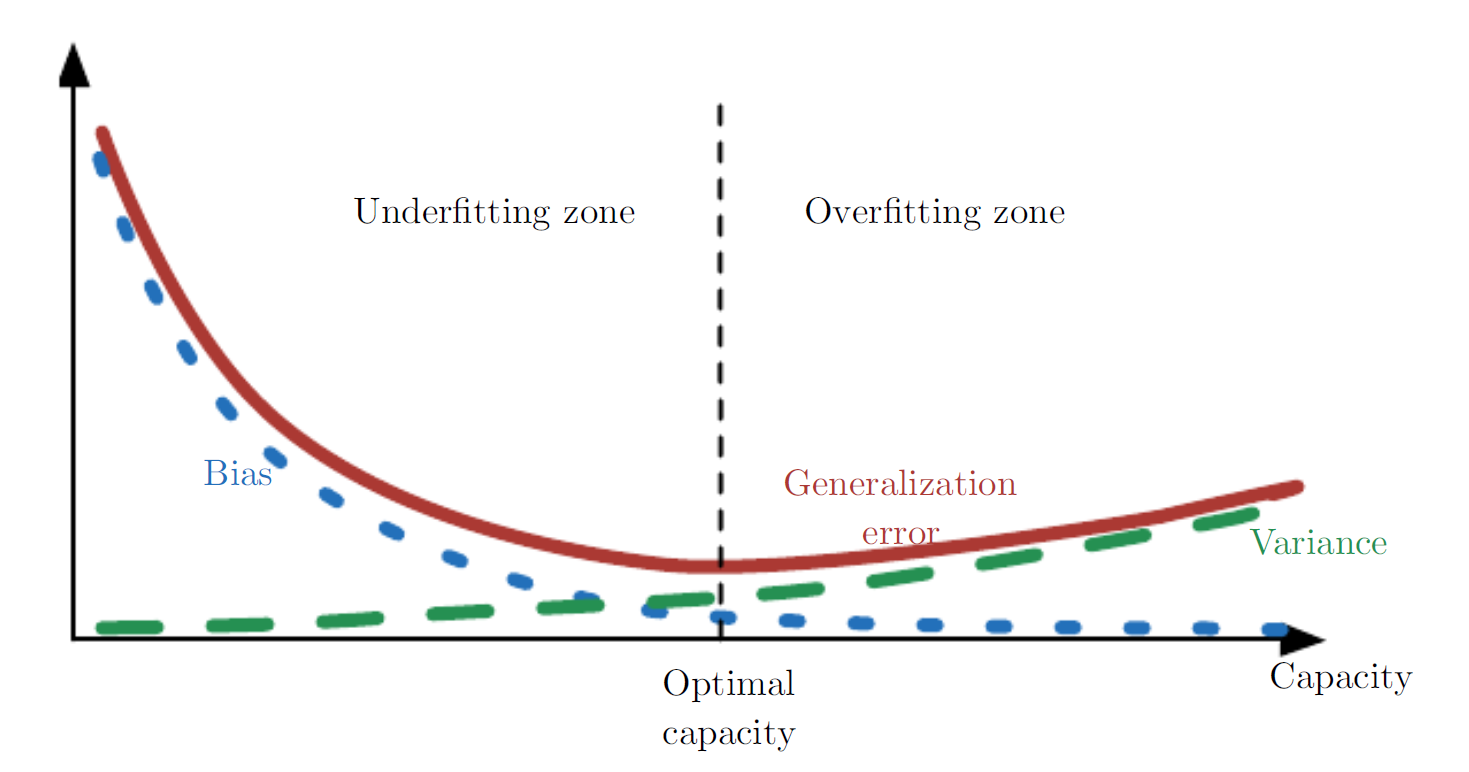
\includegraphics[width=0.7\textwidth]{Images/relationship.png}
        \caption{Relationship between Bias and Variance \footnote{\fullcite{goodfellow}}}
    \end{figure}
\end{frame}

\begin{frame}{Hyper-parameters Tuning}
\begin{block}{L2 Regularization}
    \begin{itemize}
        \item It prevents the network from over-fitting on outliers 
        \item It penalize the weight matrix to prevent it from being too large
        \item The higher value of $\lambda$ is expected; however, larger than optimal value tends increase the variance  
    \end{itemize}
    \centering{
    \textbf{Cost Function:}
    $J(w, b)=\frac{1}{m} \sum_{i=1}^{m} L\left(a^{(i)}, y\right)+\frac{\lambda}{2 m}\|w\|_{2}^{2}$}\\
\end{block}   

    \begin{block}{Mini-batch Size}
        \begin{itemize}
            \item Large training dataset divided into small batches to improve the training speed
            \item Small size mini-batch training is extremely noisy and larger size tends to slower the convergence time
            \item Optimal size of mini-batch should be selected to balance between noise and speed
        \end{itemize}
    \end{block}

\end{frame}

\begin{frame}{Hyper-parameters Tuning}
    \begin{block}{Number of Epoch}
        \begin{itemize}
            \item It represents the numbers of time the complete dataset passes through the network during training
            \item It should be large enough that allows an algorithm to run until sufficient accuracy is achieved.
        \end{itemize}
    \end{block}
    
        \begin{block}{Learning Rate}
         \begin{itemize}
             \item It represents the forward step size of gradient 
             \item The variation in learning rate is adopted as the training progresses to perform training on complex dataset
             \item \textbf{Warming-up}- Rate is initially low and increases exponentially till the preset value 
             \item \textbf{Learning Rate Decay}- At the final stage, rate reduces gradually or in discrete steps  
         \end{itemize}
    \end{block}   
\end{frame}

%---------------------------------------------------------

%%%%%%%YOLO Algorithm%%%%%%%%

\section{YOLO Algorithm}

%---------------------------------------------------------
\begin{frame}{YOLO Algorithm}
\begin{columns}
\column{0.6\textwidth}
\begin{figure}
    \centering
    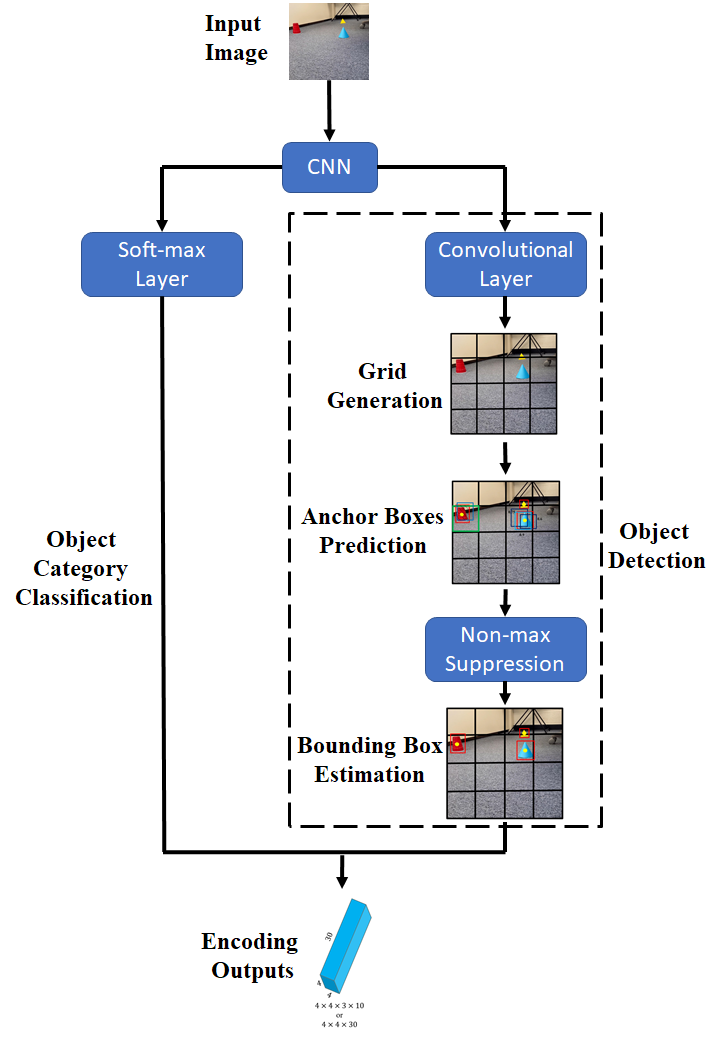
\includegraphics[width=0.78\textwidth]{Images/YOLO.png}
\end{figure}
\column{0.35\textwidth}
\begin{figure}
    \centering
    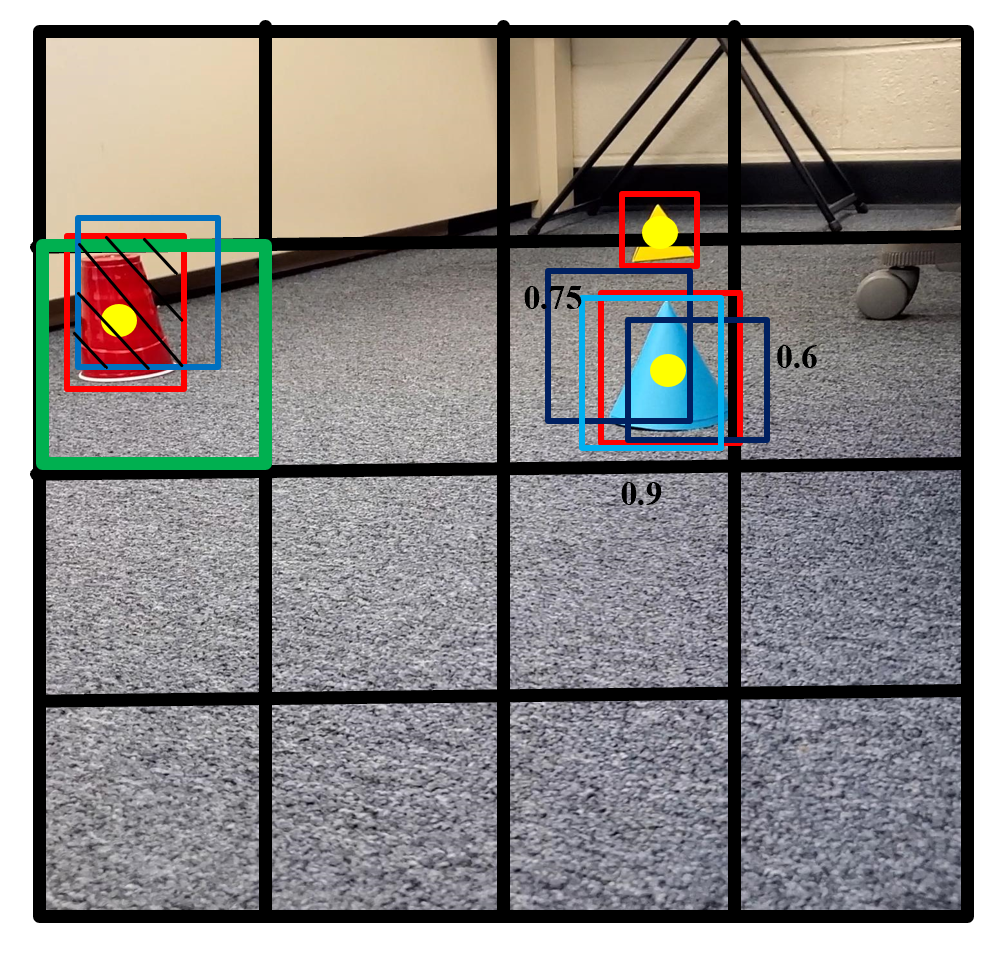
\includegraphics[width=0.9\textwidth]{Images/IOU.png}
\end{figure} 
\end{columns}
\end{frame}


%---------------------------------------------------------

%%%%%%Training Results%%%%%%%%%

\section{Training Results}

%---------------------------------------------------------
\begin{frame}{Optimal Value of Hyper-parameters}
\begin{table}
    \centering
    \begin{tabular}{|c|c|c|}
        \hline
        \textbf{Hyperparameter Name} & \textbf{Optimal Value} \\
        \hline
        Number of Iterations & 11000 \\
        \hline
        Total Number of Data & 10989\\ 
        \hline
        Learning Rate & 0.0001 \\
        \hline
        Warm-up Period & 500 iterations \\
        \hline
        L2 Regularization Parameter & 0.0005 \\
        \hline  
        Mini-batch Size & 10 \\
        \hline
        Train batch & 98\% \\
        \hline
        Test batch & 2\% \\
        \hline 
        Mean IoU of Anchor Box Estimation & 0.8738 \\
        \hline
        Number of Anchor Boxes per Detection Head & 12 \\
        \hline
    \end{tabular}
\end{table}
\end{frame}

\begin{frame}{Learning Rate \& Loss Plot}

\begin{figure}
    \centering
    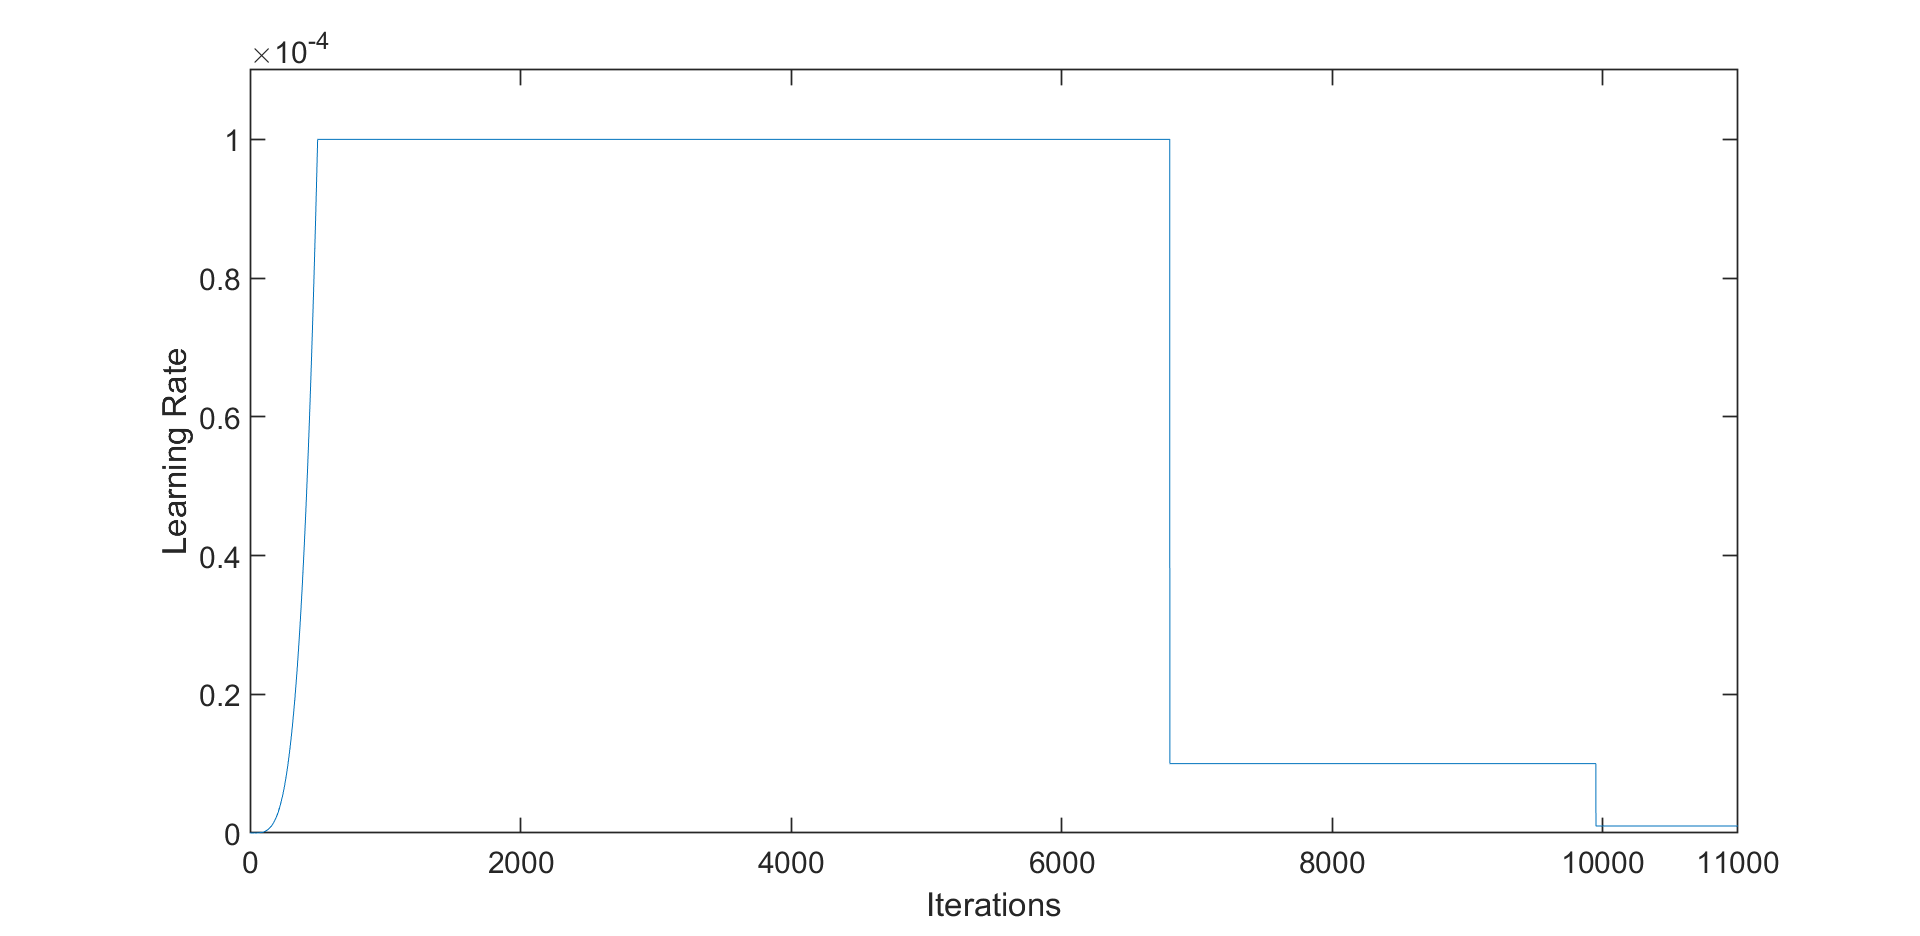
\includegraphics[width=0.6\textwidth]{Images/Learning Rate.png}
\end{figure}

\begin{figure}
    \centering
    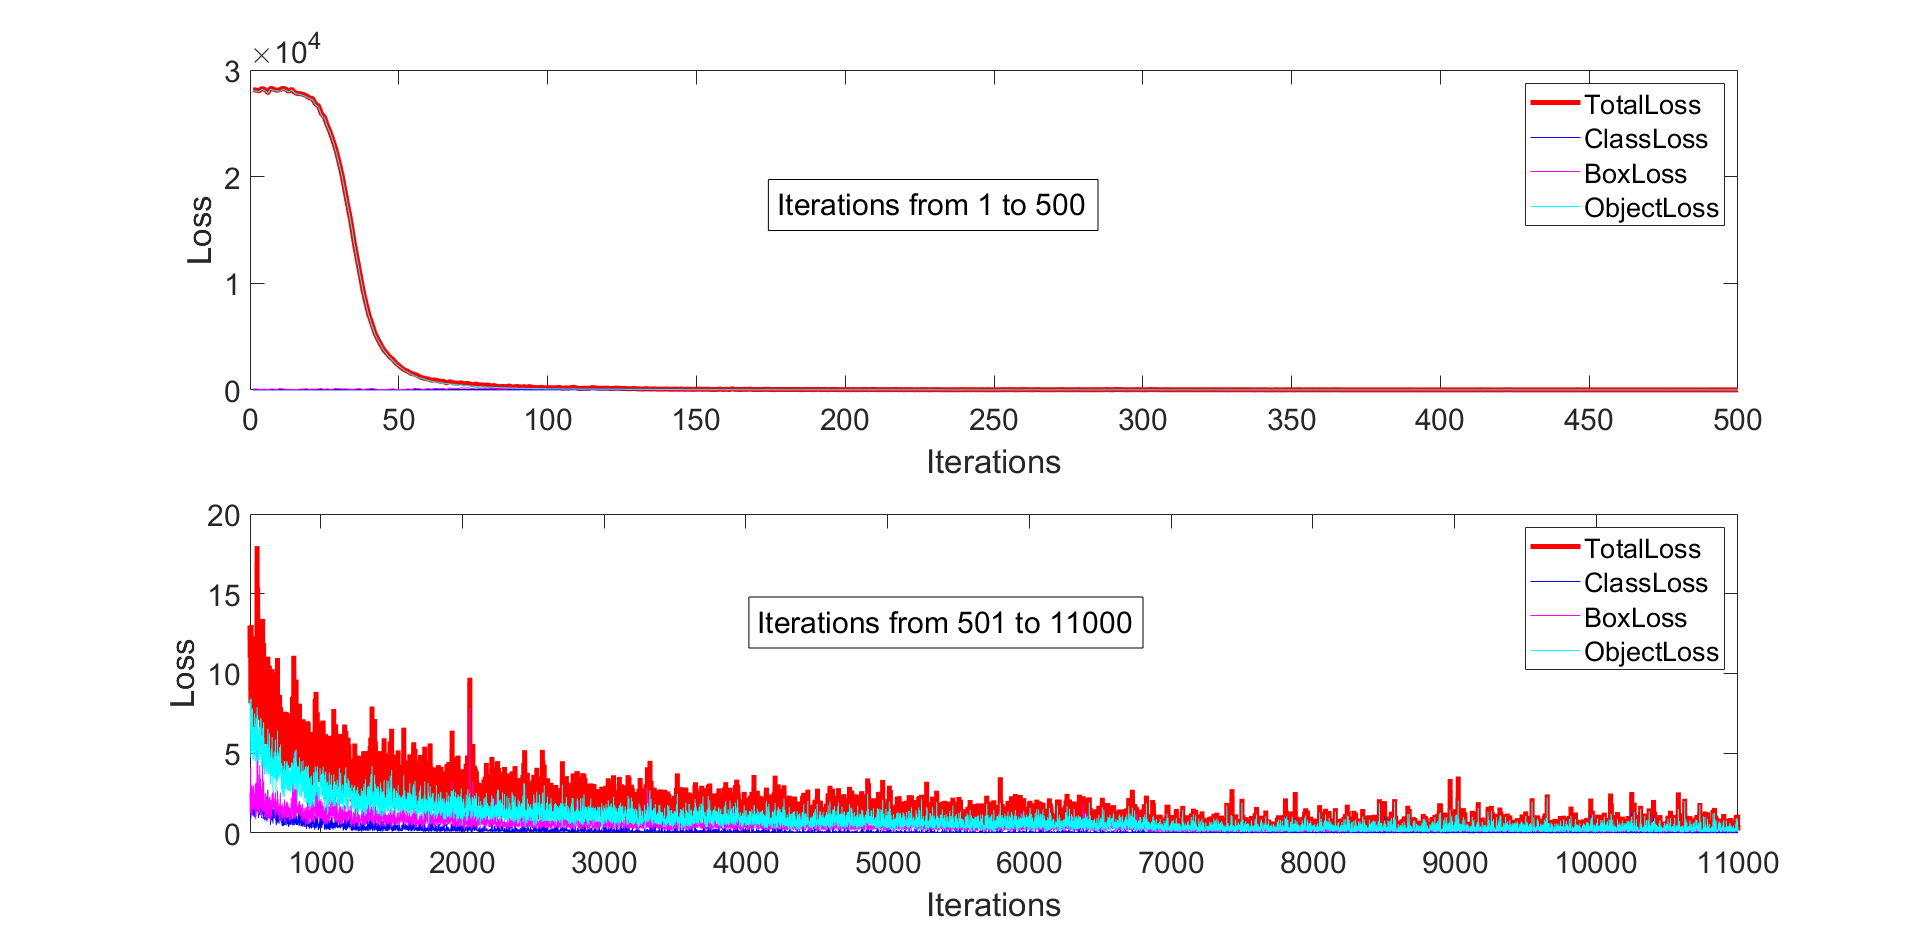
\includegraphics[width=0.6\textwidth]{Images/lossplot.png}
\end{figure}
\end{frame}

\begin{frame}{Precision Plot}
\begin{figure}
    \centering
    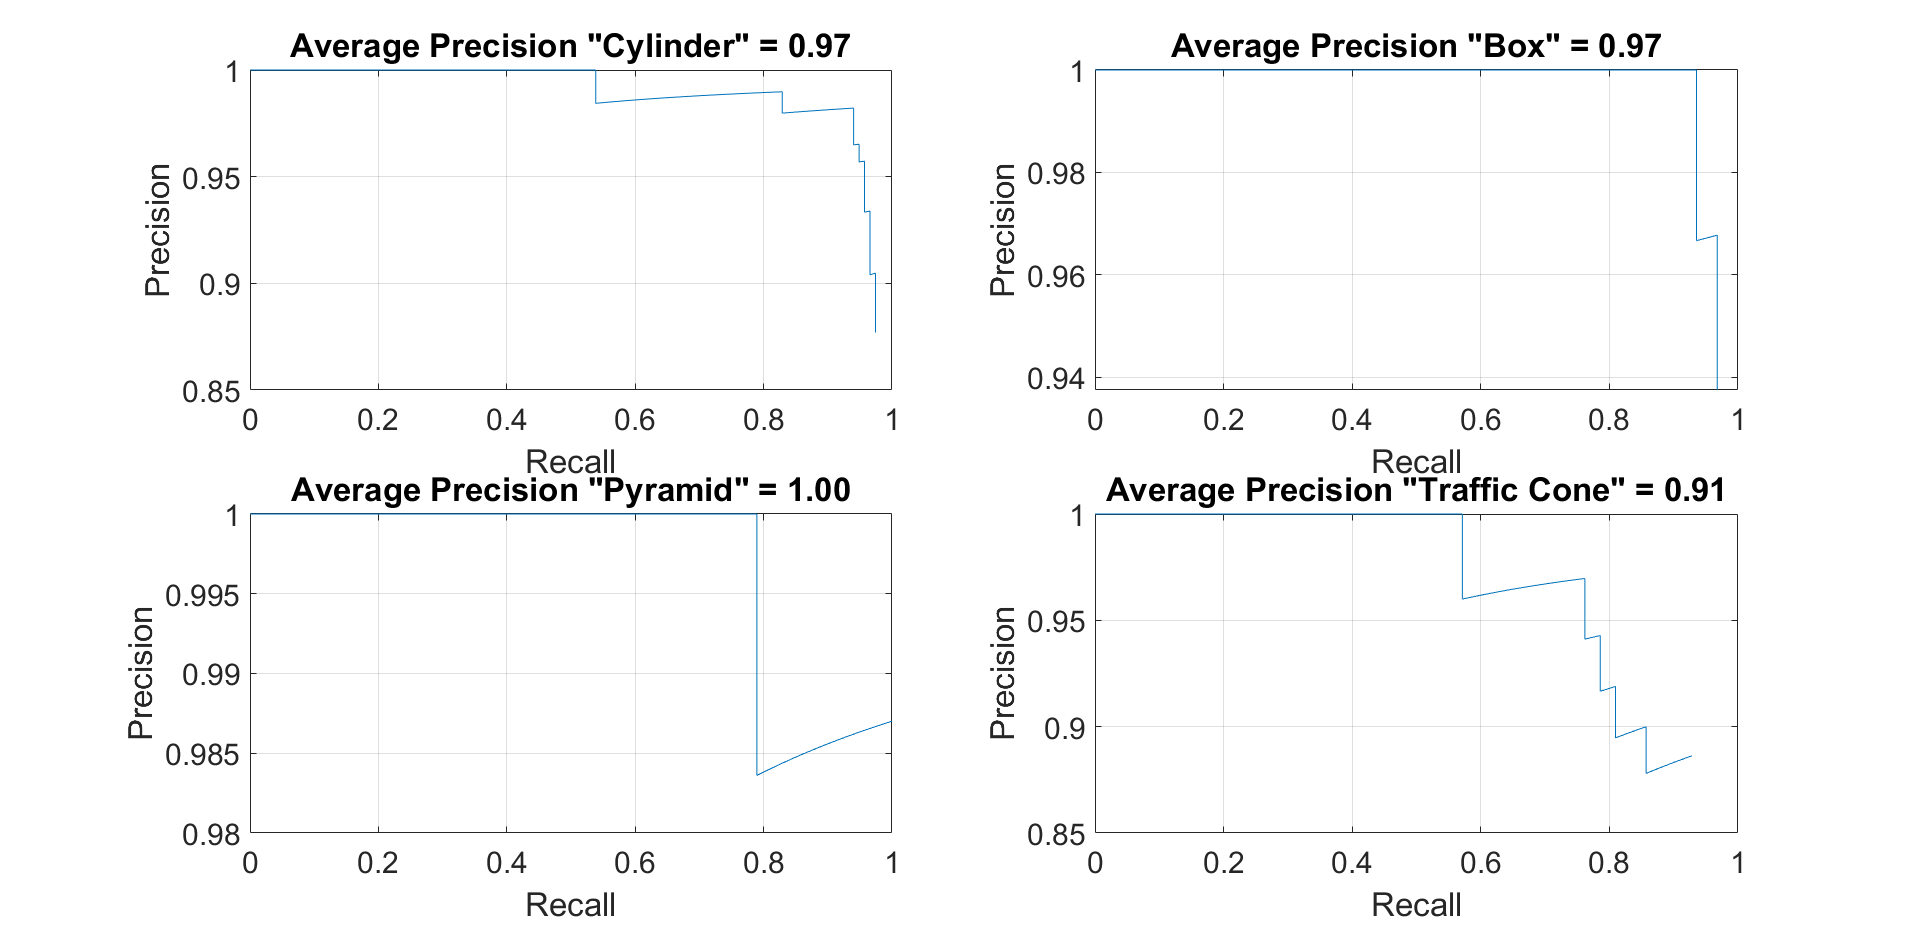
\includegraphics[width=1\textwidth]{Images/Precision_plot.png}
    \caption{Precision Plot of Test Batch}
\end{figure}
\end{frame}

\begin{frame}{Training \& Testing Performace}
\begin{table}[b]
    \centering
    \begin{tabular}{|c|c|}
        \hline
        \textbf{Parameter} & \textbf{Worth} \\
        \hline
        Average Detection Time & 59 ms\\
        \hline
        mean IoU & 0.8157\\
        \hline
        Training Accuracy & 99.08\% \\
        \hline
        Testing Accuracy & 96.25\% \\
        \hline  
    \end{tabular}
    \caption{Performance Parameters of Training \& Testing}
\end{table}
\end{frame}

\begin{frame}{Pie-Chart}
\begin{figure}
    \centering
    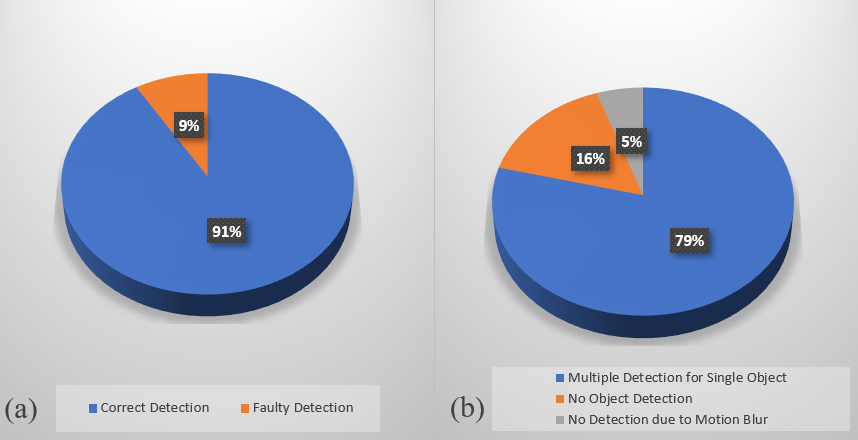
\includegraphics[width=0.9\textwidth]{Images/piechart.png}
    \caption{Pie Chart of Test Results}
\end{figure}
\end{frame}

\begin{frame}{Object Detection Results}
\begin{columns}
     \column{0.3\textwidth}
     \begin{figure}
         \centering
         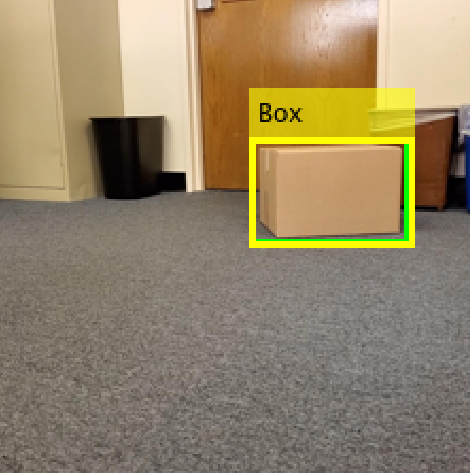
\includegraphics[width=0.75\textwidth]{Images/tt1.png}
         \caption{a}
     \end{figure}
     \vspace{-10pt}
     \begin{figure}
         \centering
         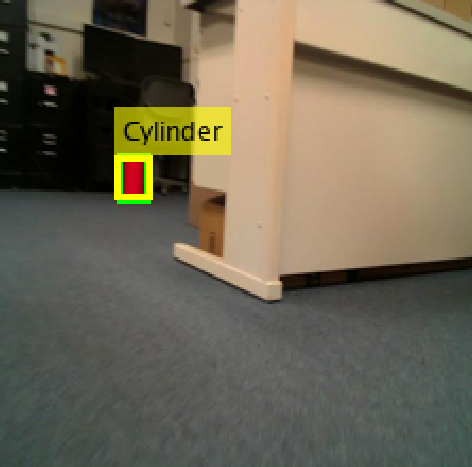
\includegraphics[width=0.75\textwidth]{Images/tt2.png}
         \caption{b}
     \end{figure}  
     \column{0.3\textwidth}
     \begin{figure}
         \centering
         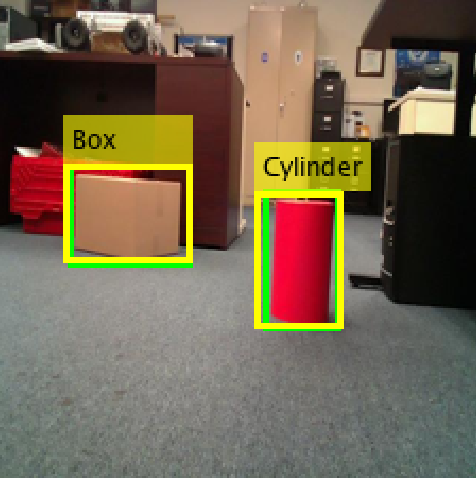
\includegraphics[width=0.75\textwidth]{Images/tt3.png}
         \caption{c}
     \end{figure}
     \vspace{-10pt}
     \begin{figure}
         \centering
         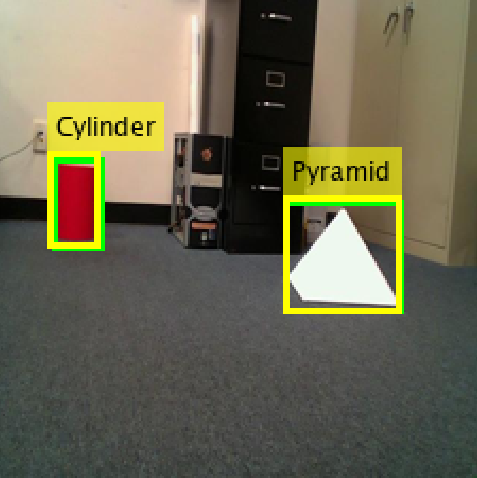
\includegraphics[width=0.75\textwidth]{Images/tt4.png}
         \caption{d}
     \end{figure}
     \column{0.3\textwidth}
     \begin{figure}
         \centering
         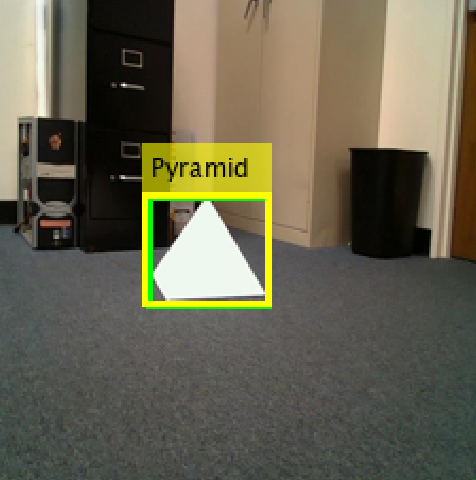
\includegraphics[width=0.75\textwidth]{Images/tt5.png}
         \caption{e}
     \end{figure}
     \vspace{-10pt}
     \begin{figure}
         \centering
         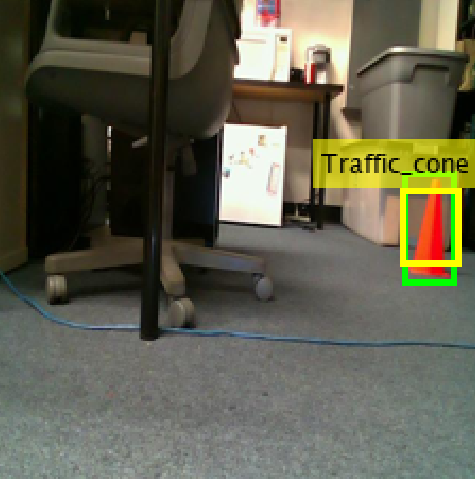
\includegraphics[width=0.75\textwidth]{Images/tt6.png}
         \caption{f}
     \end{figure}  
\end{columns}   
\end{frame}


\begin{frame}{Faulty Detections}
\begin{columns}
     \column{0.3\textwidth}
     \begin{figure}
         \centering
         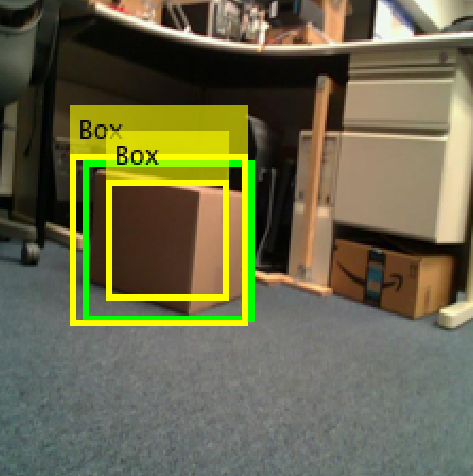
\includegraphics[width=0.7\textwidth]{Images/ft1.png}
         \caption{Multiple Detection for Single Object}
     \end{figure}
     \vspace{-20pt}
     \begin{figure}
         \centering
         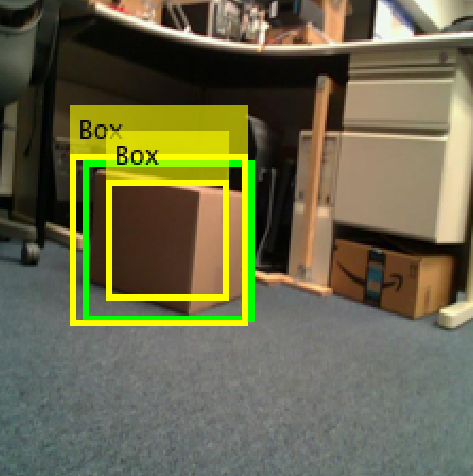
\includegraphics[width=0.7\textwidth]{Images/ft1.png}
         \caption{Multiple Detection for Single Object}
     \end{figure}  
     \column{0.3\textwidth}
     \begin{figure}
         \centering
         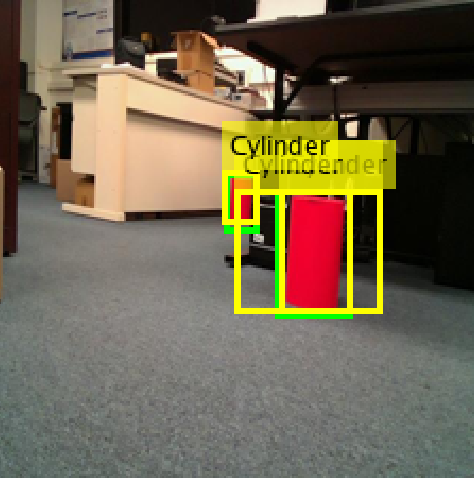
\includegraphics[width=0.7\textwidth]{Images/ft3.png}
         \caption{Multiple Detection for Single Object}
     \end{figure}
     \vspace{-20pt}
     \begin{figure}
         \centering
         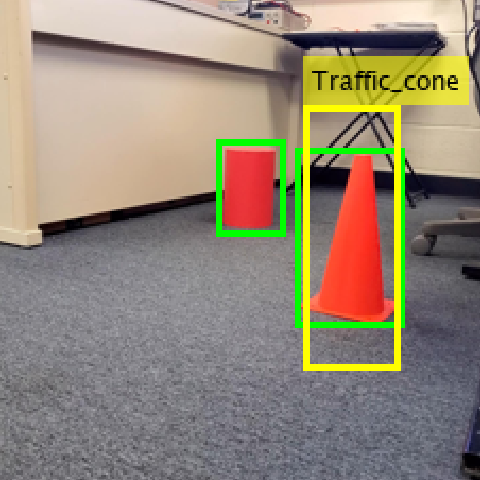
\includegraphics[width=0.7\textwidth]{Images/ft4.png}
         \caption{No Detection}
     \end{figure}
     \column{0.3\textwidth}
     \begin{figure}
         \centering
         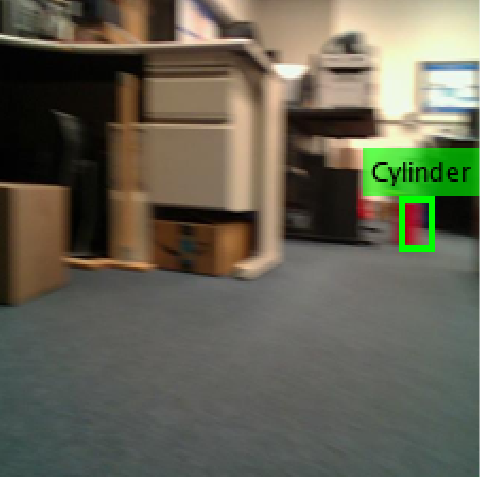
\includegraphics[width=0.7\textwidth]{Images/ft5.png}
         \caption{No Detection due to Motion Blur}
     \end{figure}
     \vspace{-20pt}
     \begin{figure}
         \centering
         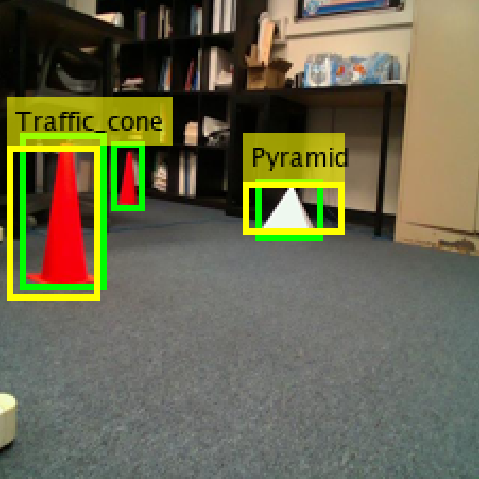
\includegraphics[width=0.7\textwidth]{Images/ft6.png}
         \caption{No Detection}
     \end{figure}  
\end{columns} 
\end{frame}

%---------------------------------------------------------

%%%%%%Optical Sensor \& Calibration%%%%%%%%%

\section{Optical Sensor \& Calibration}

%---------------------------------------------------------
\begin{frame}{Single Pin-hole Camera Model}


$$\left[\begin{array}{ccc}
x \\
y \\
1
\end{array}\right] 
 = K \times 
\left[\begin{array}{ccc}
R & t
\end{array}\right] 
 \times
\left[\begin{array}{ccc}
X \\
Y \\
Z \\
1
\end{array}\right]  
\hspace{-4pt}
K = \left[\begin{array}{ccc}f_{x} & 0 & 0 \\ s & f_{y} & 0 \\ c_{x} & c_{y} & 1\end{array}\right]$$ 


Where, K is a intrinsic matrix, R and t are rotation and translation matrices, $(f_{x},f_{y})$ is a focal length in pixel, $(c_{x},c_{y})$ is optical center coordinates in pixel, and s is skew coefficient.   
  

\begin{figure}
    \centering
    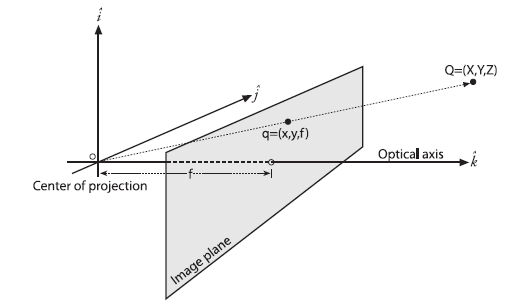
\includegraphics[width= 0.4\textwidth]{Images/pinhole.png}
    \caption{Single Pin-hole Camera Model \footnote{\fullcite{opencv}}}
\end{figure}    
\end{frame}

\begin{frame}{Stereo Camera}
   \begin{block}{1:Undistortion}
     \begin{itemize}
         \item Two types of distortion in camera: Radial and Tangential
         \item Light rays at the edge of a lens bend much more compare to rays close to the lens optical center which results in radial distortion
         \item Tangential distortion occurs when the lens plane is not completely parallel with the image plane 
     \end{itemize}
   \end{block}
   
   \begin{columns}
   \column{0.45\textwidth} 
   \begin{block}{2:Rectification}
       \begin{itemize}
           \item Images from two camera sensors are rotated and twisted to make the difference between their y coordinates to zero
           \item It is required when two cameras are not aligned and their image plane are not co-planner
       \end{itemize}
   \end{block}
   \column{0.45\textwidth}
   \begin{block}{3:Correspondence Formation}
       \begin{itemize}
           \item A search algorithm is used that finds similar features in both images
           \item Final outcome is disparity map which is difference between x pixel coordinate of two image
       \end{itemize}
   \end{block}
\end{columns}
\end{frame}

\begin{frame}{Stereo Camera}

    \begin{block}{4:Triangulation}
       \begin{itemize}
           \item Depth information is derived by use of disparity and distance between two cameras
           \item Depth is inversely proportional to the disparity
       \end{itemize}
    \centering
    $Z = \frac{f \cdot T}{x^l - x^r}$
       
    Where, Z is a depth of object, f is a focal length, T is a distance between two cameras, and $x^l$ and $x^r$ are the projection of object P on the left and right camera image plane respectively
       
    \begin{figure}
        \centering
        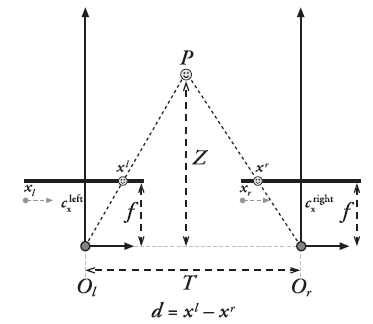
\includegraphics[width=0.35\textwidth]{Images/triangulate.png}
    \end{figure}
   \end{block}
\end{frame}

\begin{frame}{Optical sensor}
   \begin{columns}
      \column{0.45\textwidth}
      \begin{block}{Sony IMX 179}
         \centering
         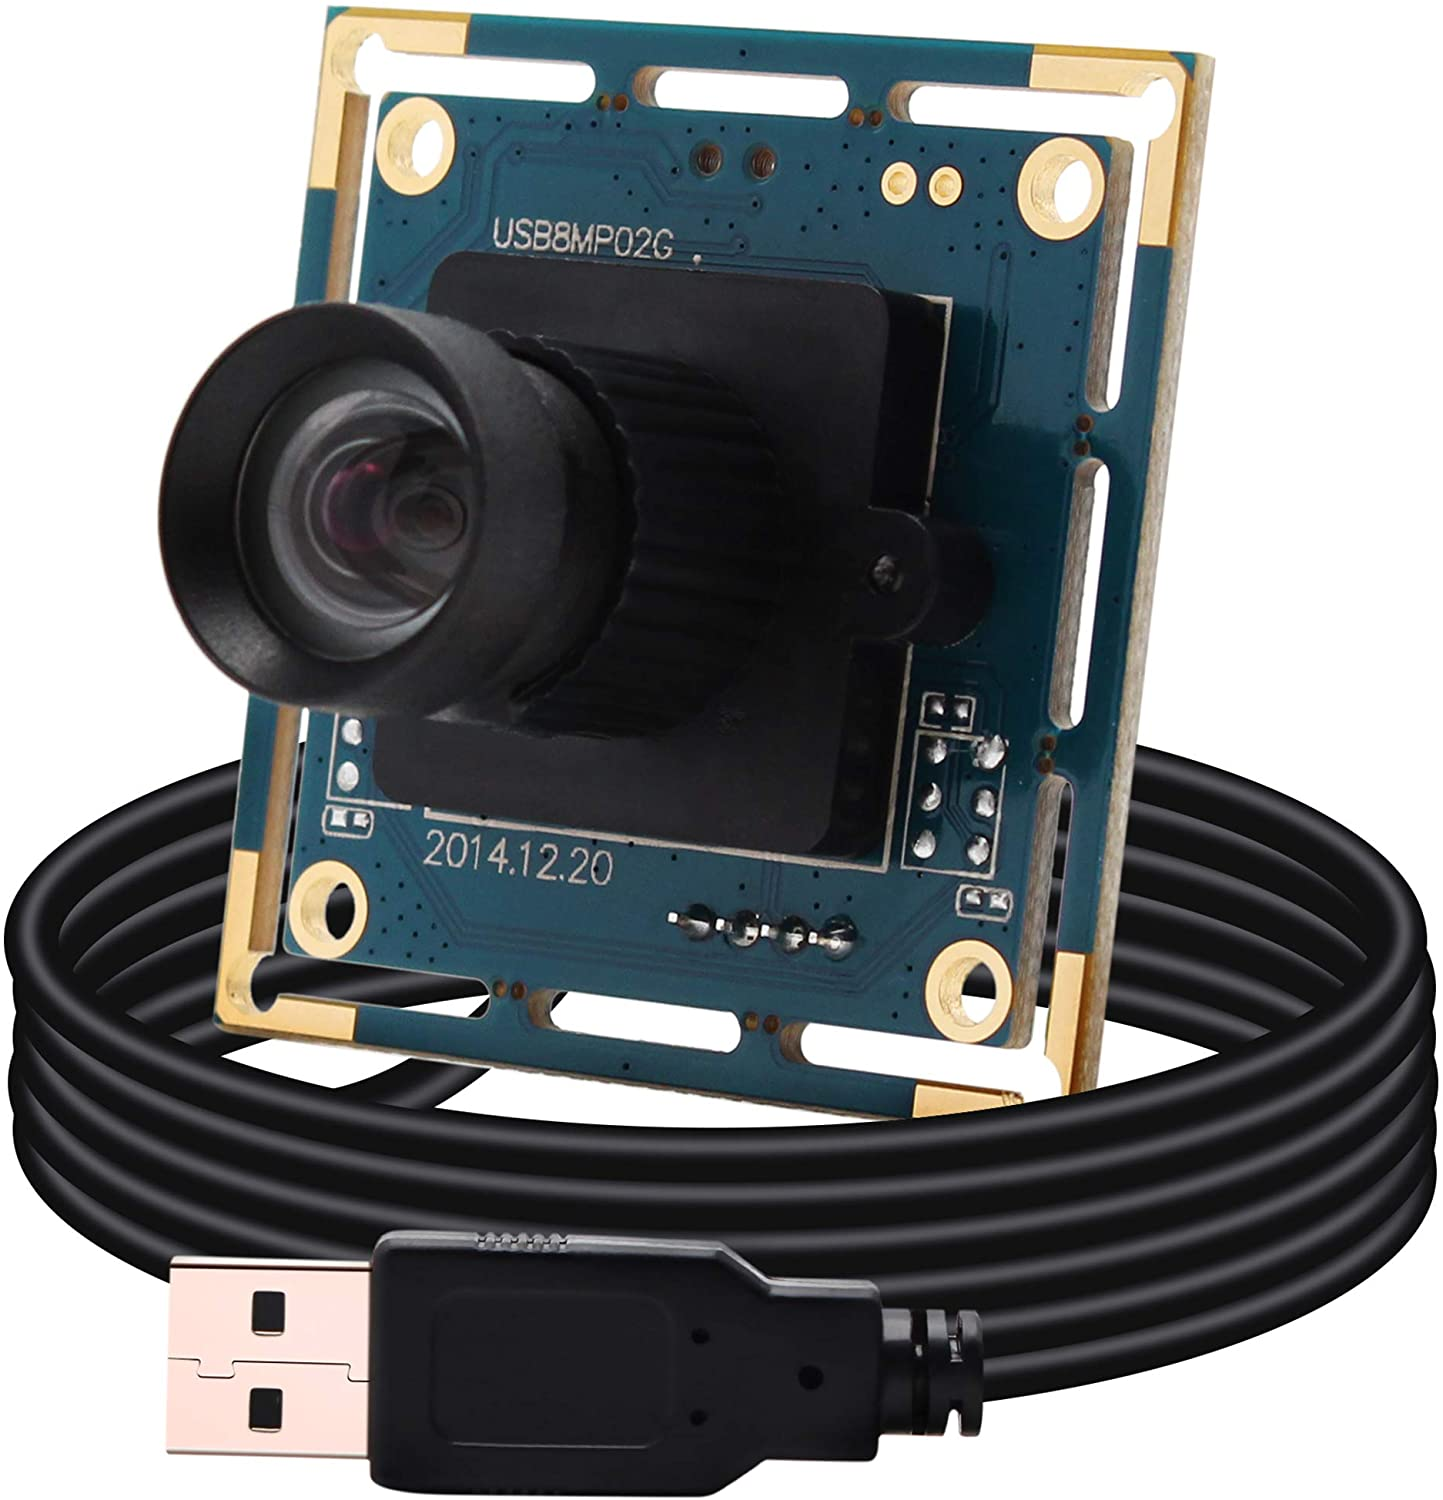
\includegraphics[width=0.5\textwidth]{Images/imx179.png}
         
        \begin{itemize}
            \item Non-distortion lens with $75^o$ horizontal field of view
            \item Max. 30 fps in all pixel scan mode
            \item 8 MP high definition resolution 
            \item Image Resolutions available: 3264 X 2448, 3200 X 2400, 1024 X 768, 1600 X 1200
        \end{itemize}
      \end{block}
      
      \column{0.45\textwidth}
      \begin{block}{Intel Realsense L515 LiDAR}
         \centering
         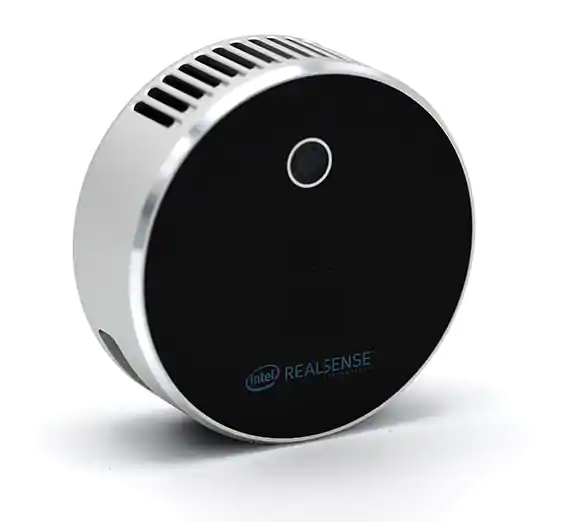
\includegraphics[width=0.6\textwidth]{Images/L515.png}
        
        \begin{itemize}
             \item A laser exposure time is less than 100 ns per depth point
             \item A number of depth points per second is 9.2 M at 640 X 480 and 23.6 M at 1024 X 768 image resolution
             \item Depth accuracy is 5 mm to 14 mm
        \end{itemize}    
      \end{block}
   \end{columns}
\end{frame}

\begin{frame}{Standard Calibration Error}
\begin{table}
    \centering
    \begin{tabular}{|l|c|c|}
        \hline
        Description & Stereo Camera & Lidar \\
        \hline
        X Error & 0.08 mm & 0.10 mm \\
        \hline
        Y Error & -0.09 mm & -0.04 mm \\ 
        \hline
        Z Error & -0.03 mm  & -0.19 mm \\
        \hline
    \end{tabular}
    \caption{Measurement Error in Intrinsic Calibration}
\end{table}

\begin{table}
    \centering
    \begin{tabular}{|l|c|c|}
        \hline
        Description & Camera to Lidar & Lidar to Camera \\
        \hline
        Transformation Error & 29.5 mm & -29.42 mm \\
        \hline
    \end{tabular}
    \caption{Transformation Error in Extrinsic Calibration}
\end{table}
\end{frame}

\begin{frame}{Real-time Object Detection Results and Position Estimation}
\begin{columns}
     \column{0.3\textwidth}
     \begin{figure}
         \centering
         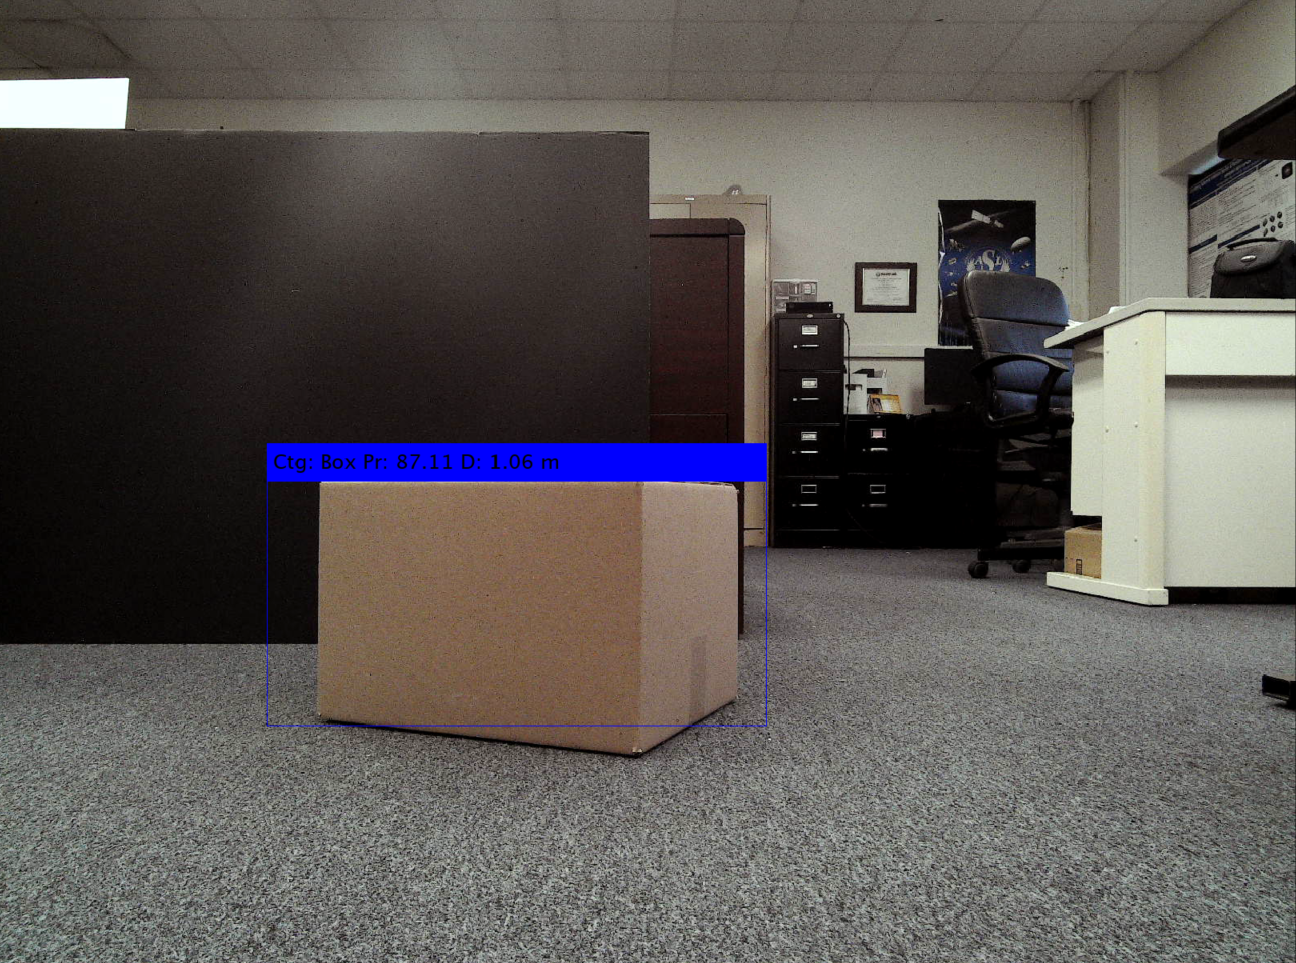
\includegraphics[width=0.8\textwidth]{Images/Box_d100cm.PNG}
         \caption{a}
     \end{figure}
     \vspace{-20pt}
     \begin{figure}
         \centering
         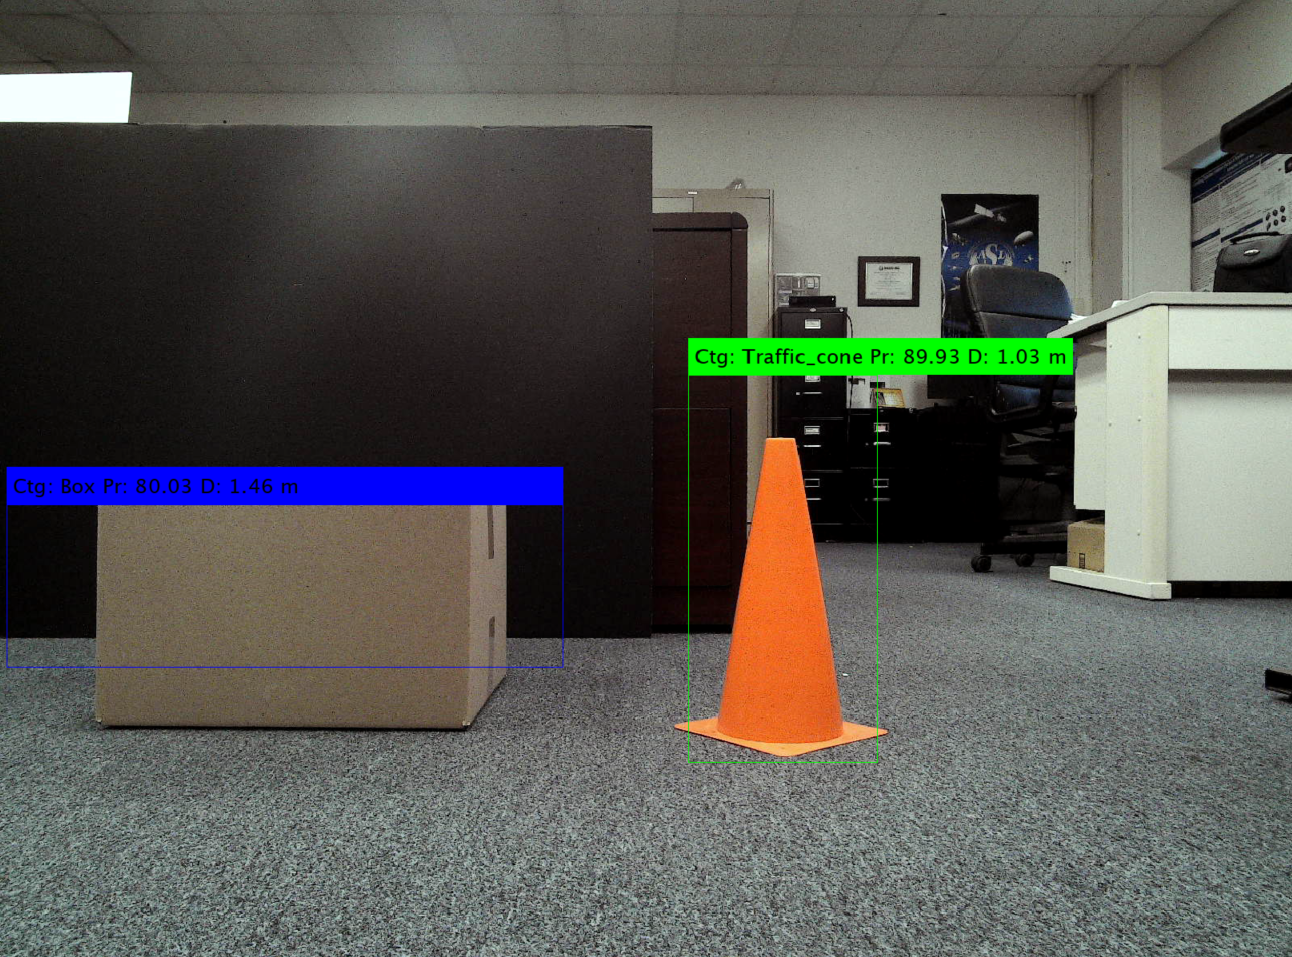
\includegraphics[width=0.8\textwidth]{Images/box_d120cm_py_d105cm.PNG}
         \caption{b}
     \end{figure}  
     \column{0.3\textwidth}
     \begin{figure}
         \centering
         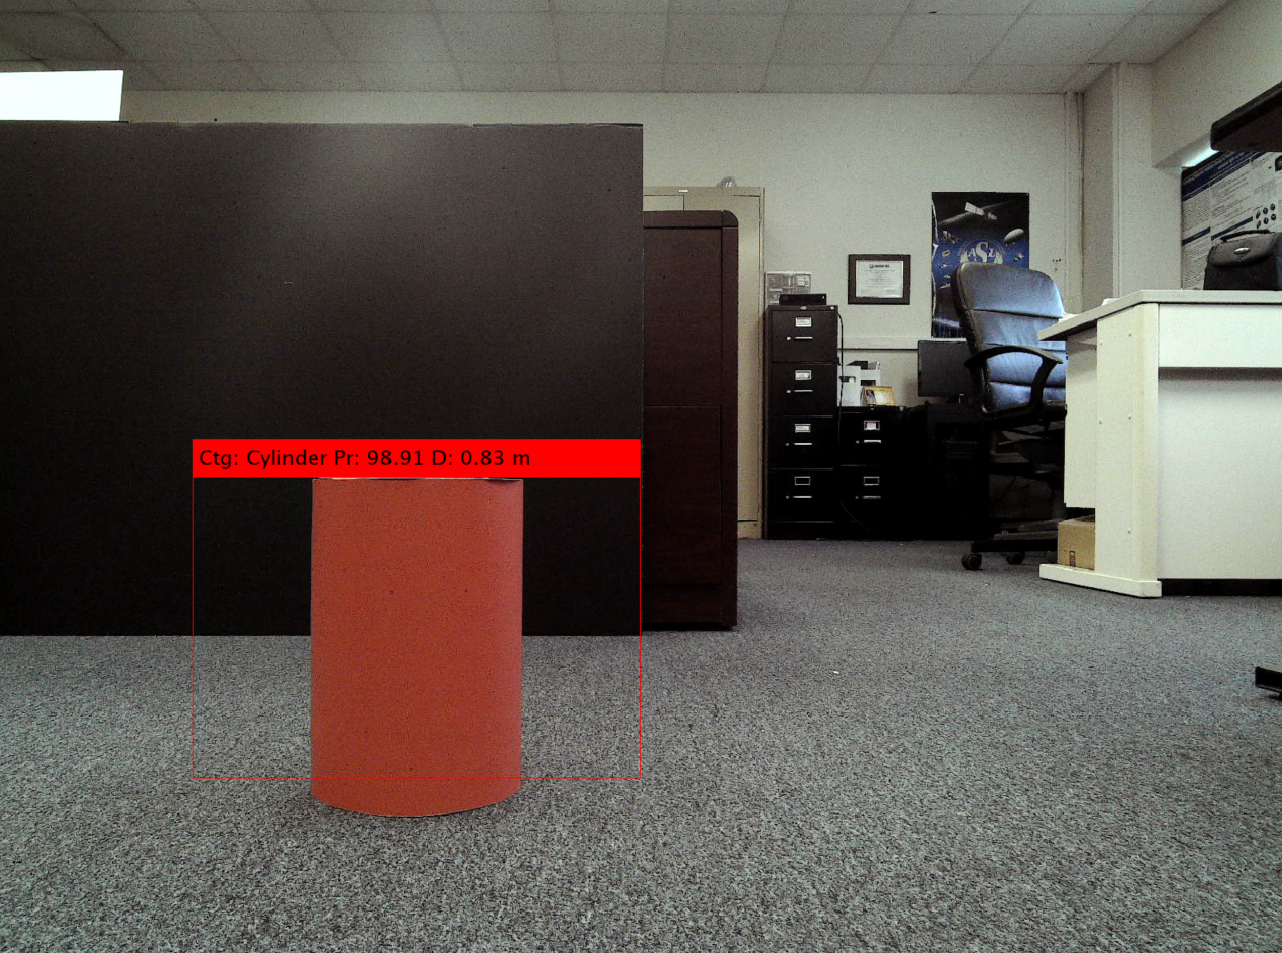
\includegraphics[width=0.8\textwidth]{Images/cy_d80cm.PNG}
         \caption{c}
     \end{figure}
     \vspace{-20pt}
     \begin{figure}
         \centering
         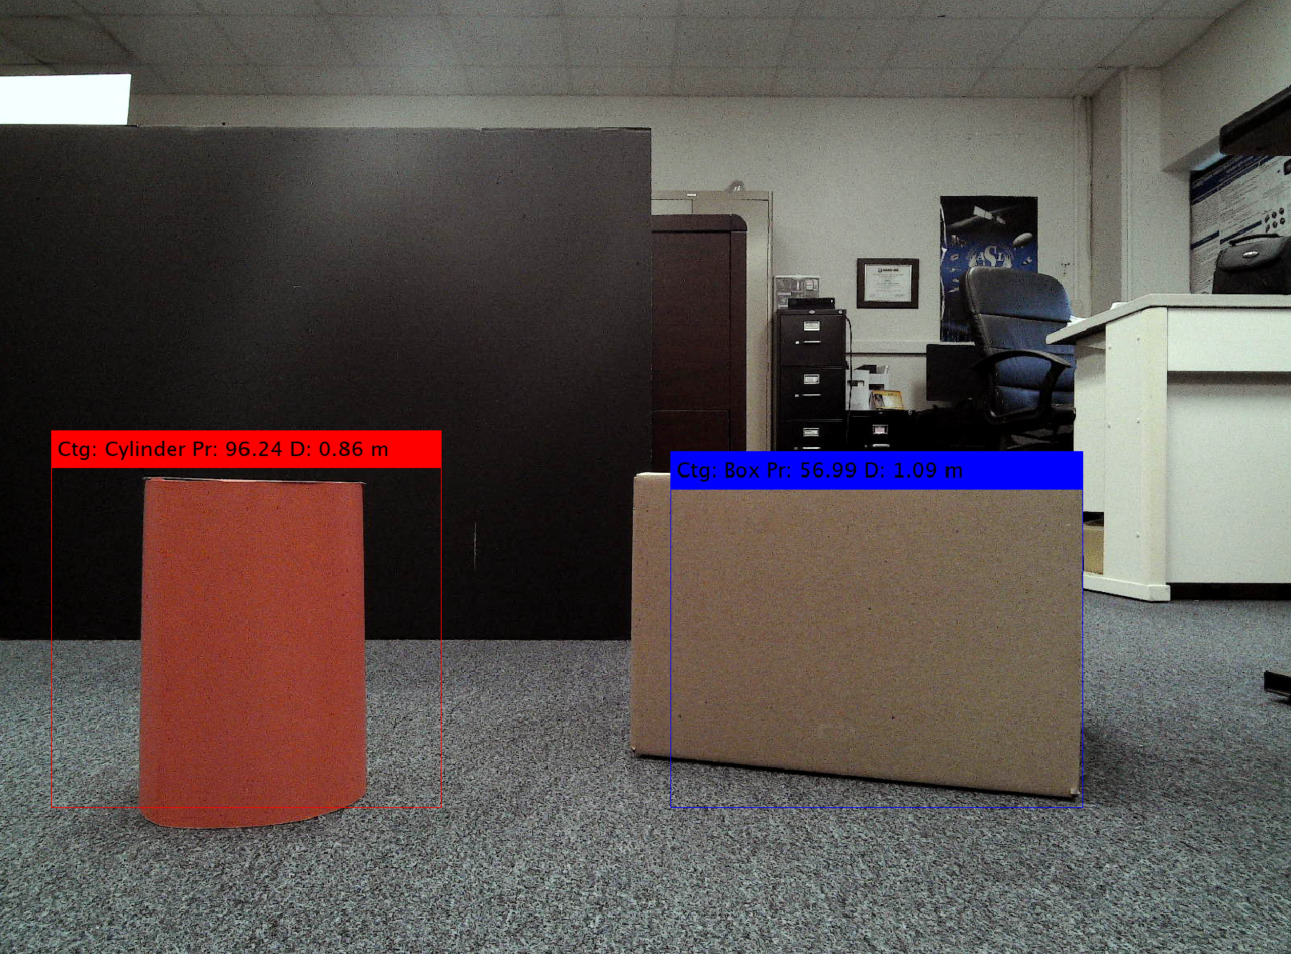
\includegraphics[width=0.8\textwidth]{Images/cy_d85cm_box_d95cm.PNG}
         \caption{d}
     \end{figure}
     \column{0.3\textwidth}
     \begin{figure}
         \centering
         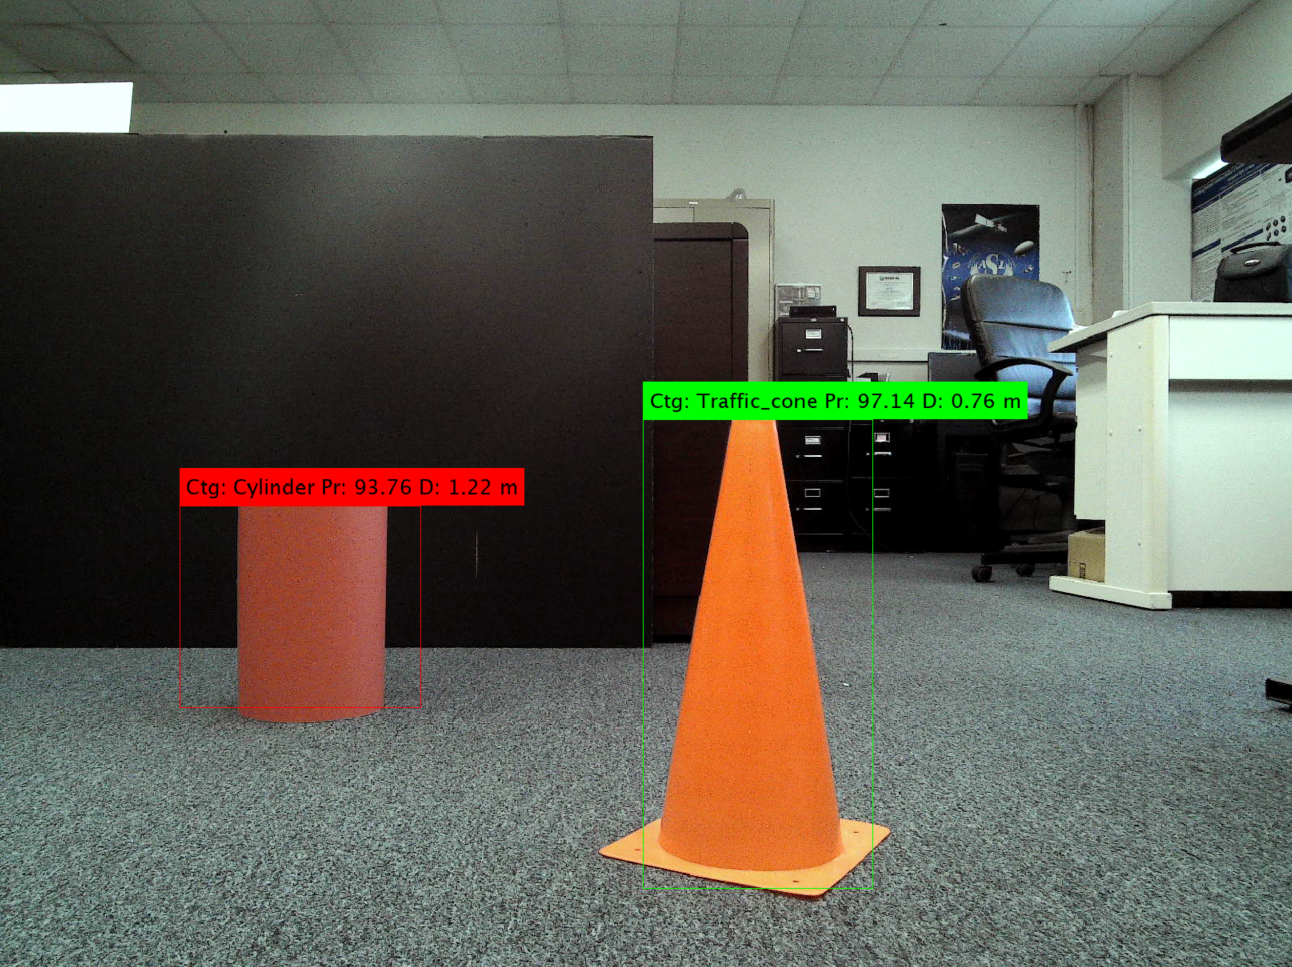
\includegraphics[width=0.8\textwidth]{Images/cy_d120cm_TC_d70cm.PNG}
         \caption{e}
     \end{figure}
     \vspace{-20pt}
     \begin{figure}
         \centering
         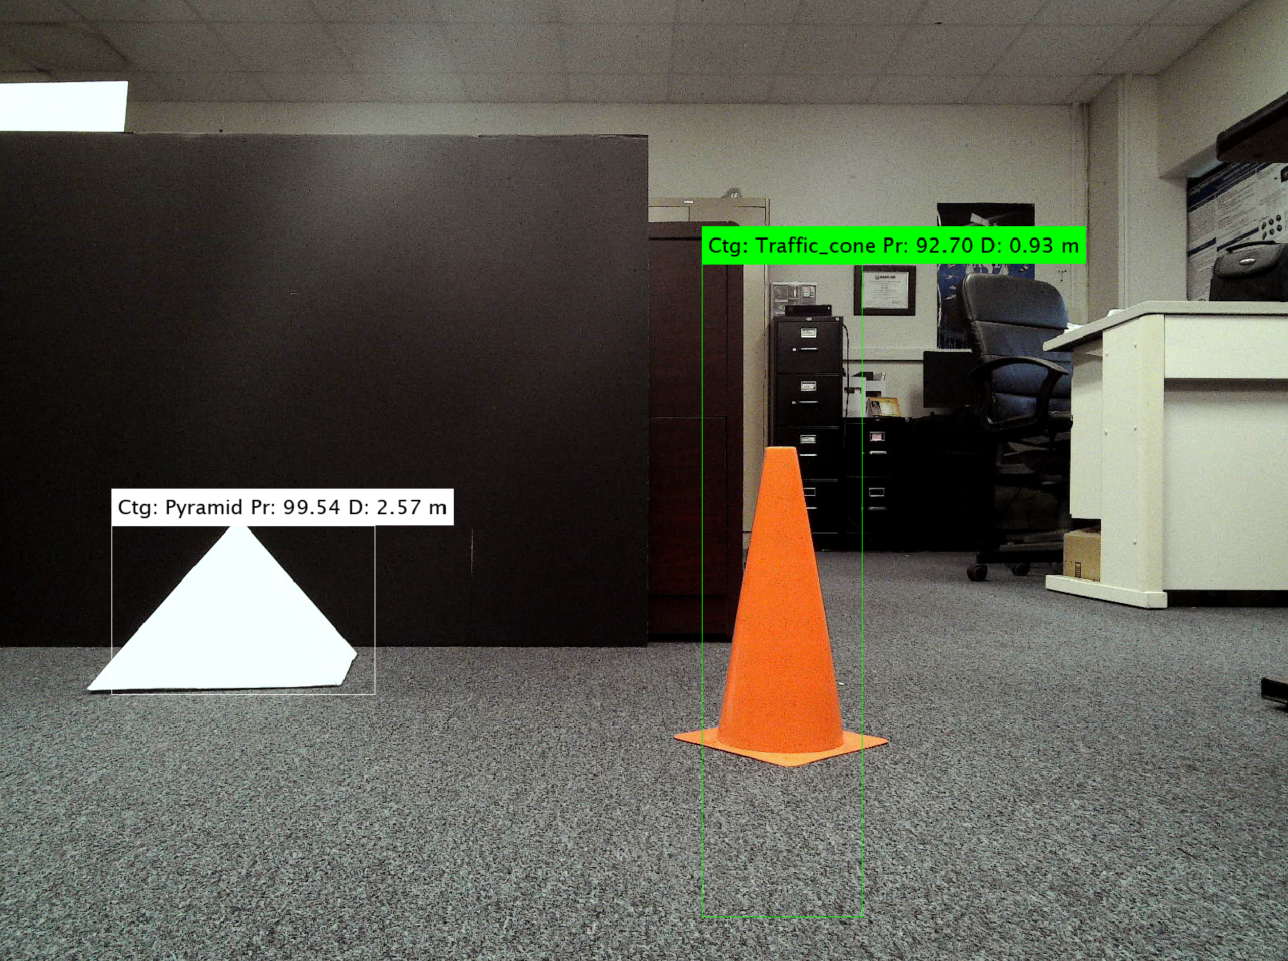
\includegraphics[width=0.8\textwidth]{Images/TC_d105cm_py_d155cm.PNG}
         \caption{f}
     \end{figure}  
\end{columns}     
\end{frame}

%---------------------------------------------------------

%%%%%%Sensor Fusion%%%%%%%%%

\section{Sensor Fusion}

%---------------------------------------------------------
\begin{frame}{Linear Kalman Filtering}
   \begin{columns}
        \column{0.43\textwidth}
        \begin{block}{System \& Measurement Model}
          \centering
          $x_{k}=F_{k-1} x_{k-1}+G_{k-1} u_{k-1}+w_{k-1}$\\
          $z_{k}=H_{k} x_{k}+v_{k}$ 
        \end{block}
        \begin{block}{Process Covariance}
              $$Q_{k} = 
                 \left[\begin{array}{ccc}
                      q_{xx} & 0 & 0 \\
                      0 & q_{yy} & 0 \\
                      0 & 0 & q_{zz}
                      \end{array}\right]$$
        \end{block}
        \begin{block}{Measurement Covariance}
              $$    R_{k} =
                    \left[\begin{array}{ccc}
                          r_{xx} & 0 & 0 \\
                          0 & r_{yy} & 0 \\
                          0 & 0 & r_{zz}
                          \end{array}\right]$$
        \end{block}  
        
        \column{0.53\textwidth}
        \begin{block}{State Transition Metric}
        Constant Acceleration Model
        \tiny
              $$F_{k-1} =
                 \left[\begin{array}{ccccccccc}
                      1 & T & \frac{1}{2} T^2 & 0 & 0 & 0 & 0 & 0 & 0\\
                      0 & 1 & T & 0 & 0 & 0 & 0 & 0 & 0 \\
                      0 & 0 & 1 & 0 & 0 & 0 & 0 & 0 & 0\\
                      0 & 0 & 0 &  1 & T & \frac{1}{2} T^2 & 0 & 0 & 0\\
                      0 & 0 & 0 & 0 & 1 & T & 0 & 0 & 0\\
                      0 & 0 & 0 & 0 & 0 & 1 & 0 & 0 & 0\\
                      0 & 0 & 0 & 0 & 0 & 0 & 1 & T & \frac{1}{2} T^2\\
                      0 & 0 & 0 & 0 & 0 & 0 & 0 & 1 & T\\
                      0 & 0 & 0 & 0 & 0 & 0 & 0 & 0 & 1
                      \end{array}\right]$$
        \end{block}
        \begin{block}{Measurement Metric}
              $$ H_{k} =
                    \left[\begin{array}{ccccccccc}
                          1 & 0 & 0 & 0 & 0 & 0 & 0 & 0 & 0 \\
                          0 & 0 & 0 & 1 & 0 & 0 & 0 & 0 & 0 \\
                          0 & 0 & 0 & 0 & 0 & 0 & 1 & 0 & 0
                          \end{array}\right]$$
        \end{block}          
   \end{columns}
\end{frame}

\begin{frame}{Linear Kalman Filtering}

\begin{figure}
    \centering
    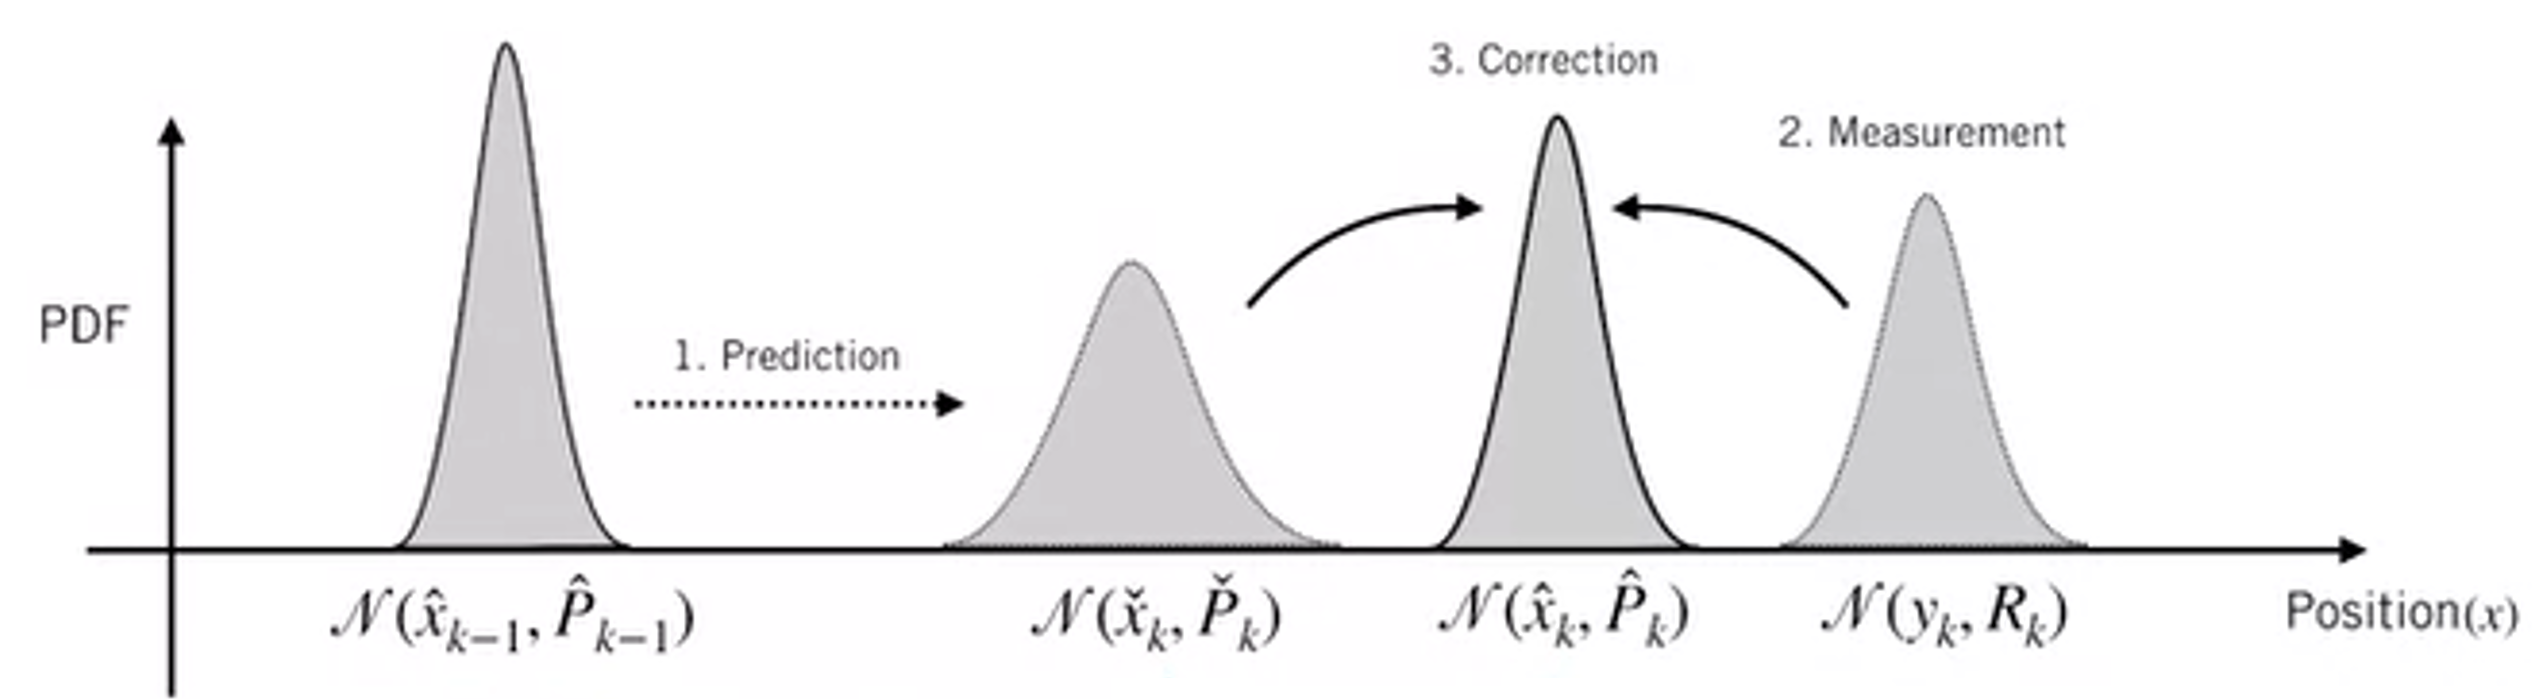
\includegraphics[width=0.5\textwidth]{Images/KF.png}
\end{figure}
 \vspace{-5pt}
   \begin{block}{Prediction}
   
      The state estimation of previous time stamp $x_{k}$ is substituted in dynamic model to propagate the state forward as $x_{k+1|k}$. \\
      \centering
       $x_{k+1 / k}=F_{k} x_{k / k}+G_{k / k} u_{k}$\\ 
       $P_{k+1 / k}=F_{k} P_{k / k} F_{k}^{T}+Q_{k}$
   \end{block}
   \vspace{-5pt}
    \begin{block}{Measurement \& Correction}
    
      The predicted states are corrected by using measurements through feedback. 
      \centering
       $K_{k+1}=P_{k+1 / k} H_{k+1}^{T}\left(H_{k+1} P_{k+1 / k} H_{k+1}^{T}+R_{k+1}\right)^{-1}$\\
      $x_{k+1 / k+1}=x_{k+1 / k}+K_{k+1}\left(\tilde{z}_{k+1}-H_{k+1} x_{k+1 / k}\right)$\\
      $P_{k+1 / k+1}=\left(1-k_{k+1} H_{k+1}\right) p_{k+1 / k}$
   \end{block}  
\end{frame}

\begin{frame}{Multi-sensor Data Fusion}
\begin{figure}
    \centering
    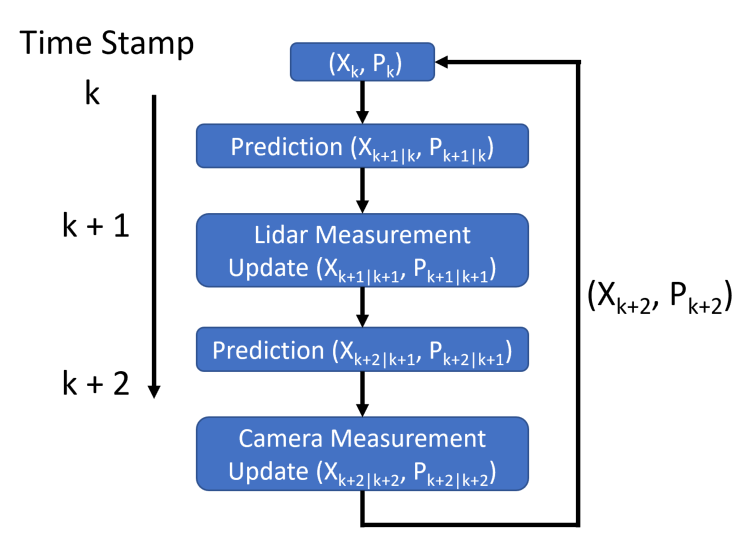
\includegraphics[width=0.75\textwidth]{Images/fusion.png}
    \caption{Flowchart of Multi-sensor Data Fusion for Asynchronous Case}
\end{figure}
\end{frame}

%---------------------------------------------------------

%%%%%%Simulation Results%%%%%%%%%

\section{Simulation Results}

%---------------------------------------------------------

\begin{frame}{Driving Scene}
  \begin{columns}
       \column{0.45\textwidth}
       \begin{figure}
           \centering
           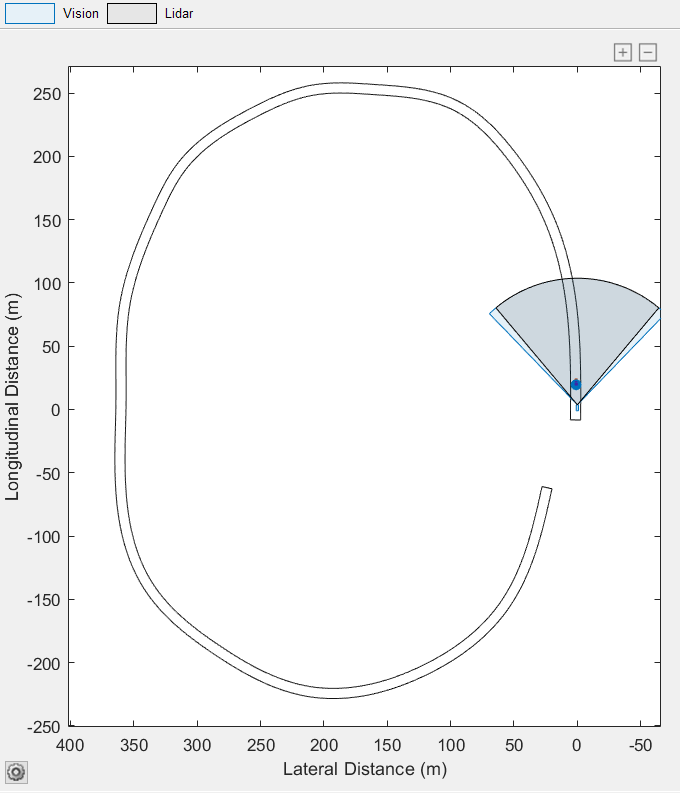
\includegraphics[width=0.45\textwidth]{Images/Drivingscene.png}
           \caption{Bird's Eye View of Scene}
       \end{figure}
       
       \column{0.45\textwidth}
       \begin{figure}
           \centering
           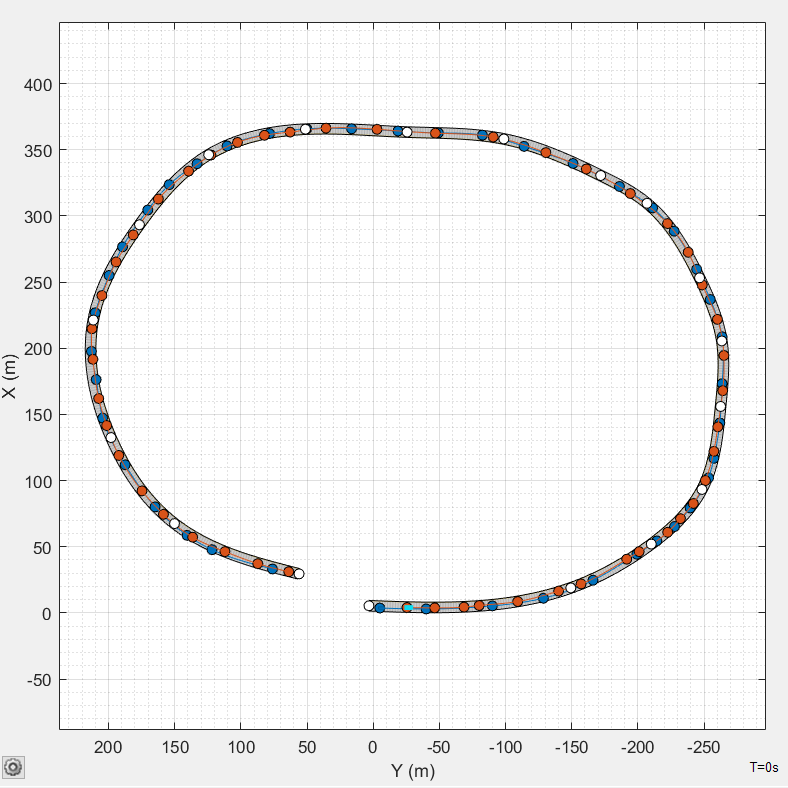
\includegraphics[width=0.5\textwidth]{Images/waypoints.png}
           \caption{Way points Definition}
       \end{figure}
  \end{columns}
  
\begin{table}
    \centering
    \begin{tabular}{|c|c|}
        \hline
        \textbf{Scene Parameter} & \textbf{Worth} \\
        \hline
        Ego Vehicle Speed & 30 m/s (67 mph)\\
        \hline
        Object Vehicle Speed & 30 m/s (67 mph)\\
        \hline
        Camera Azimuthal Limits & [-43 43] (deg) \\
        \hline
        Camera Elevation Limits & [-90 90] (deg)\\
        \hline  
        Lidar Azimuthal Limits & [-40 40] (deg)\\
        \hline
        Lidar Elevation Limits & [-90 90] (deg)\\
        \hline
    \end{tabular}
    \caption{Driving Scene Parameters}
\end{table} 
\end{frame}

\begin{frame}{Sensor Co-variance \& Measurement Error}

\begin{block}{Sensor Co-variance}
    $$R_{LiDAR} = 
    \left[\begin{array}{ccc}
    0.2102 & 0 & 0 \\
    0 & 0.0093 & 0 \\
    0 & 0 & 0.0001
    \end{array}\right]$$ \\

    $$R_{Camera} =
    \left[\begin{array}{ccc}
    1.5336 & 0 & 0 \\
    0 & 1.3365 & 0 \\
    0 & 0 & 0.0001
    \end{array}\right]$$
\end{block}

\begin{block}{Sensor Measurement Error}
\begin{table}
    \centering
    \begin{tabular}{|c|c|c|c|}
        \hline
        \textbf{Description} & \textbf{Camera} & \textbf{Lidar} & \textbf{Estimation} \\
        \hline
        X Error & 0.95 m & 0.29 m & 0.40 m\\
        \hline
        Y Error & 0.20 m & 0.033 m & 0.14 m\\
        \hline
        X Error & 0.0001 m & 0.0001 m & 0.00001 m\\
        \hline
        Overall Error & 0.97 m & 0.29 m & 0.42 m\\
        \hline        
    \end{tabular}
\end{table}
\end{block}
\end{frame}

\begin{frame}{Simulation}
 \centering
 \huge
 Video    
\end{frame}

\begin{frame}{Position Plot}
\begin{figure}
    \centering
    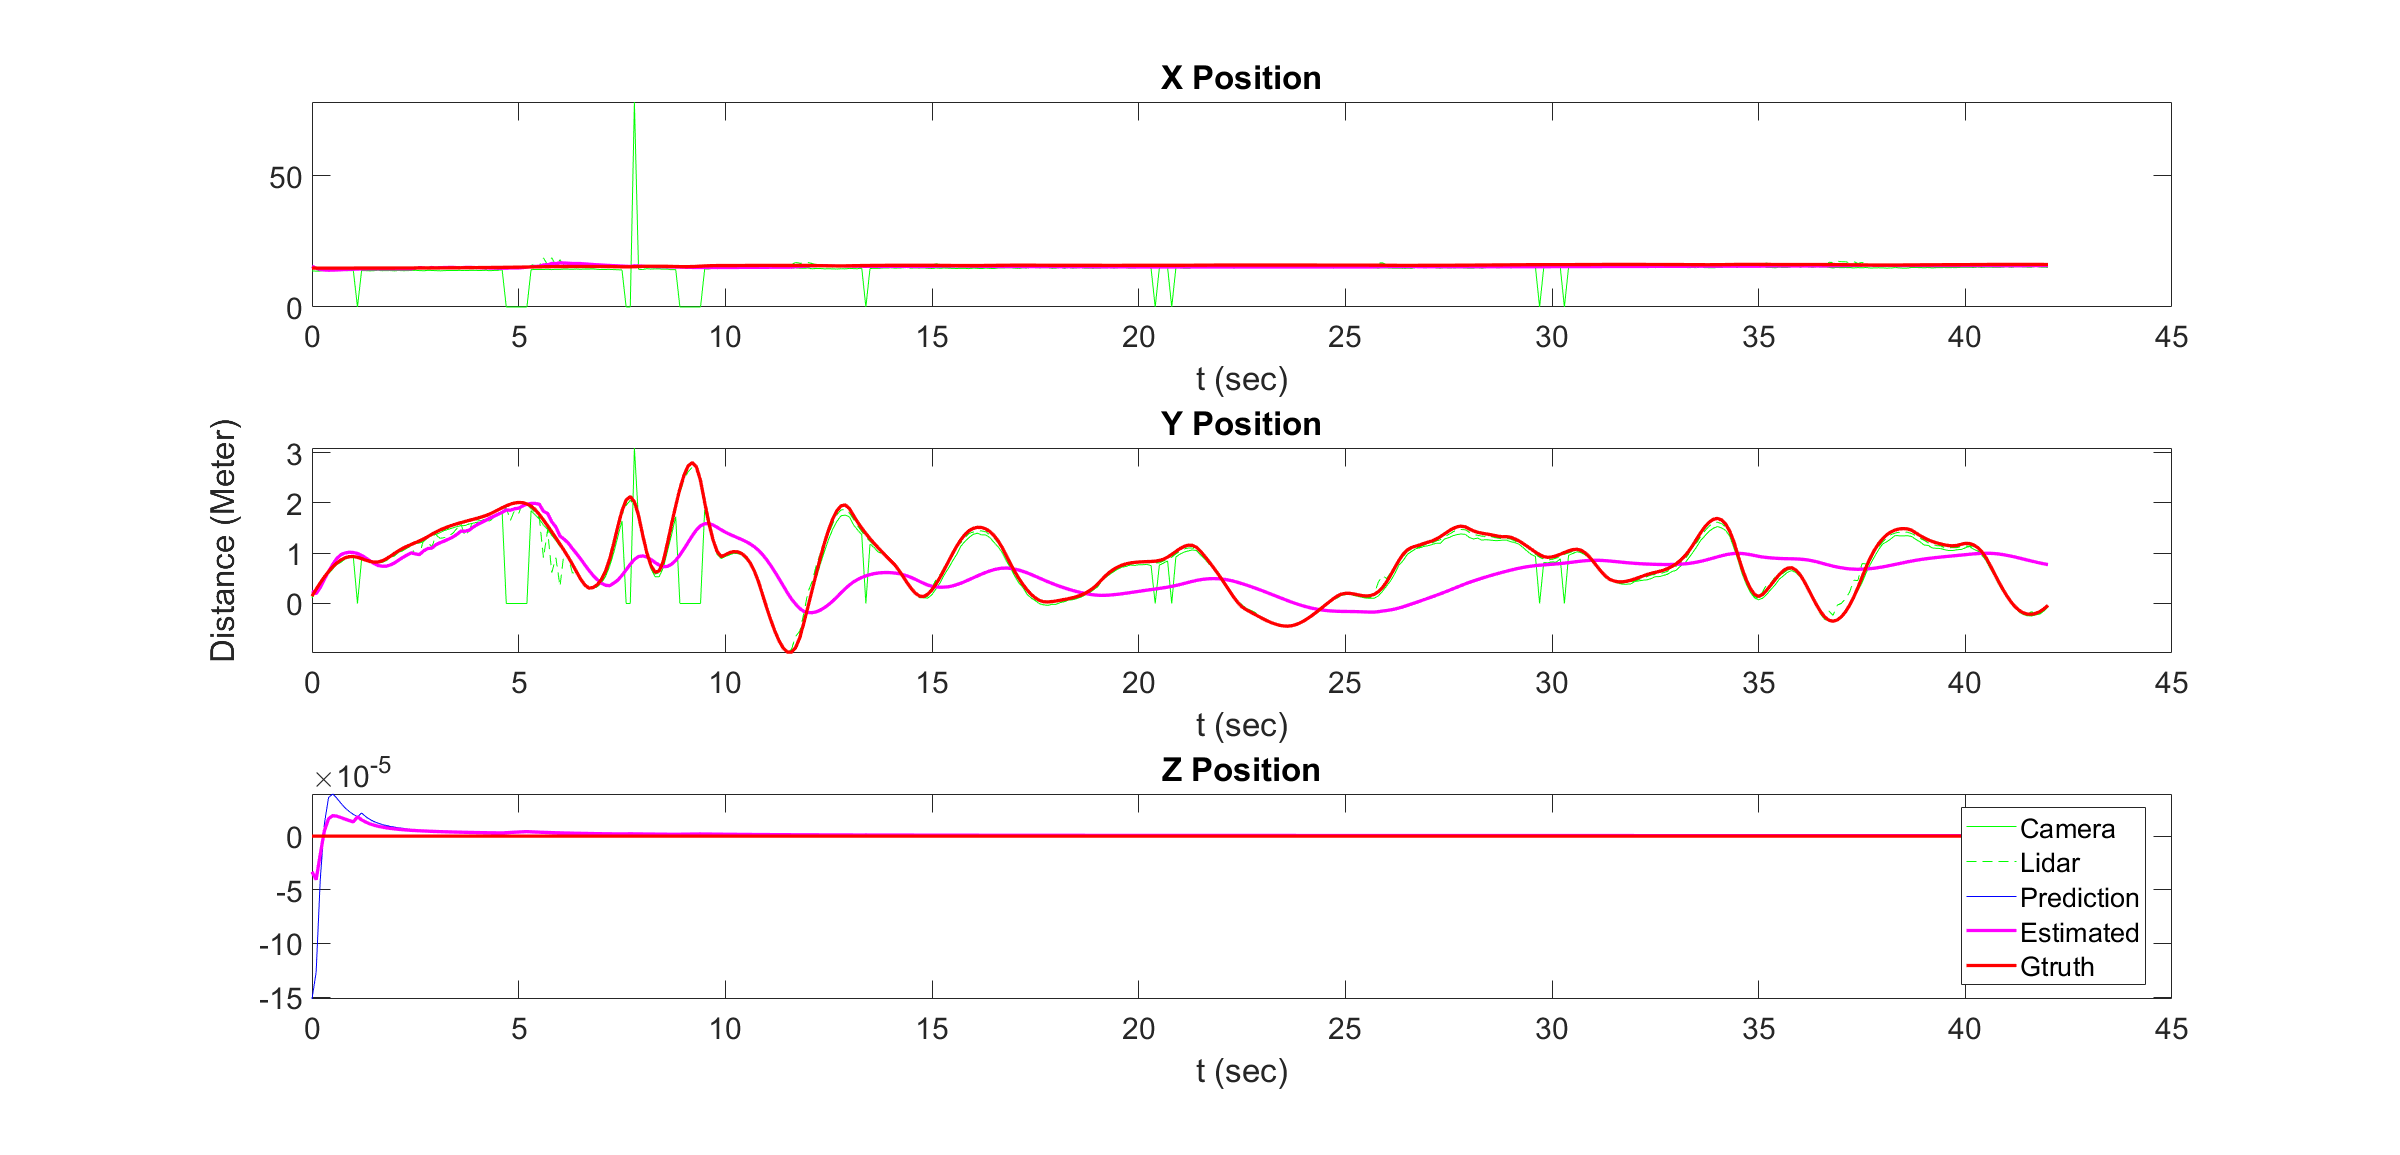
\includegraphics[width=1\textwidth]{Images/Position_plot.png}
    \caption{Position plot in Simulation}
\end{figure}
\end{frame}

\begin{frame}{Velocity Plot}
\begin{figure}
    \centering
    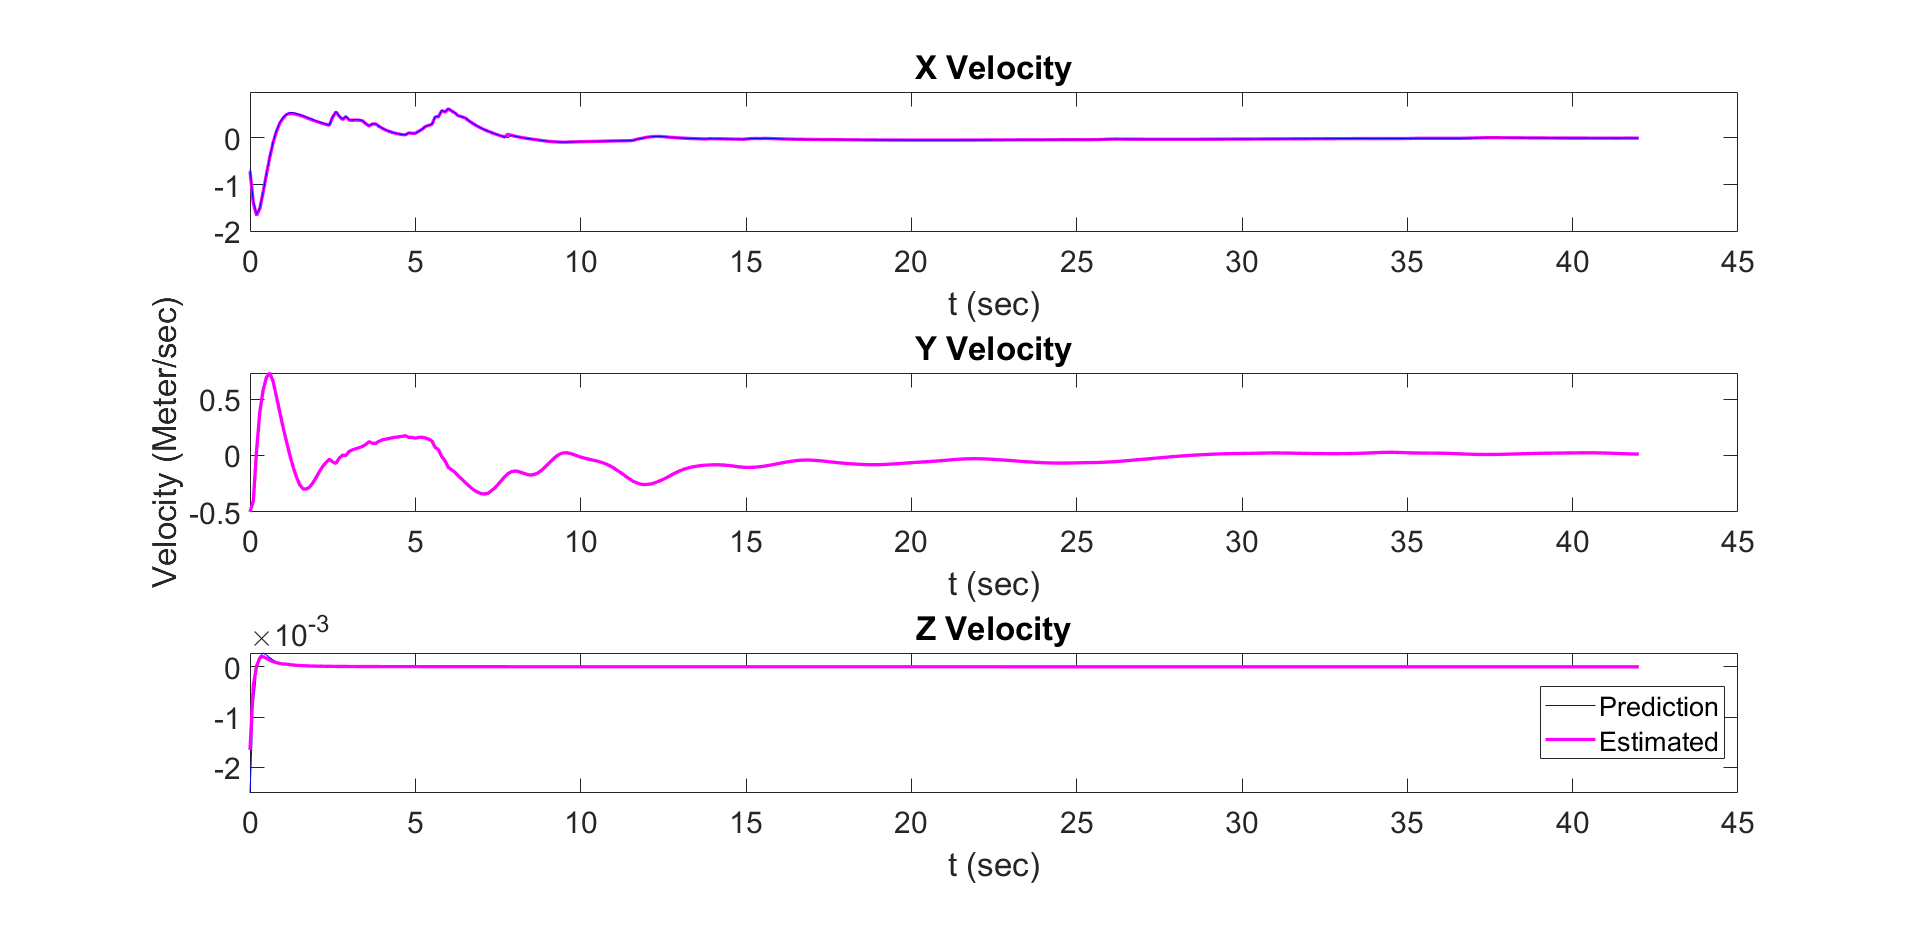
\includegraphics[width=1\textwidth]{Images/Velocity_plot.png}
    \caption{Velocity plot in Simulation}
\end{figure}
\end{frame}

\begin{frame}{Estimation Error Plot}
\begin{figure}
    \centering
    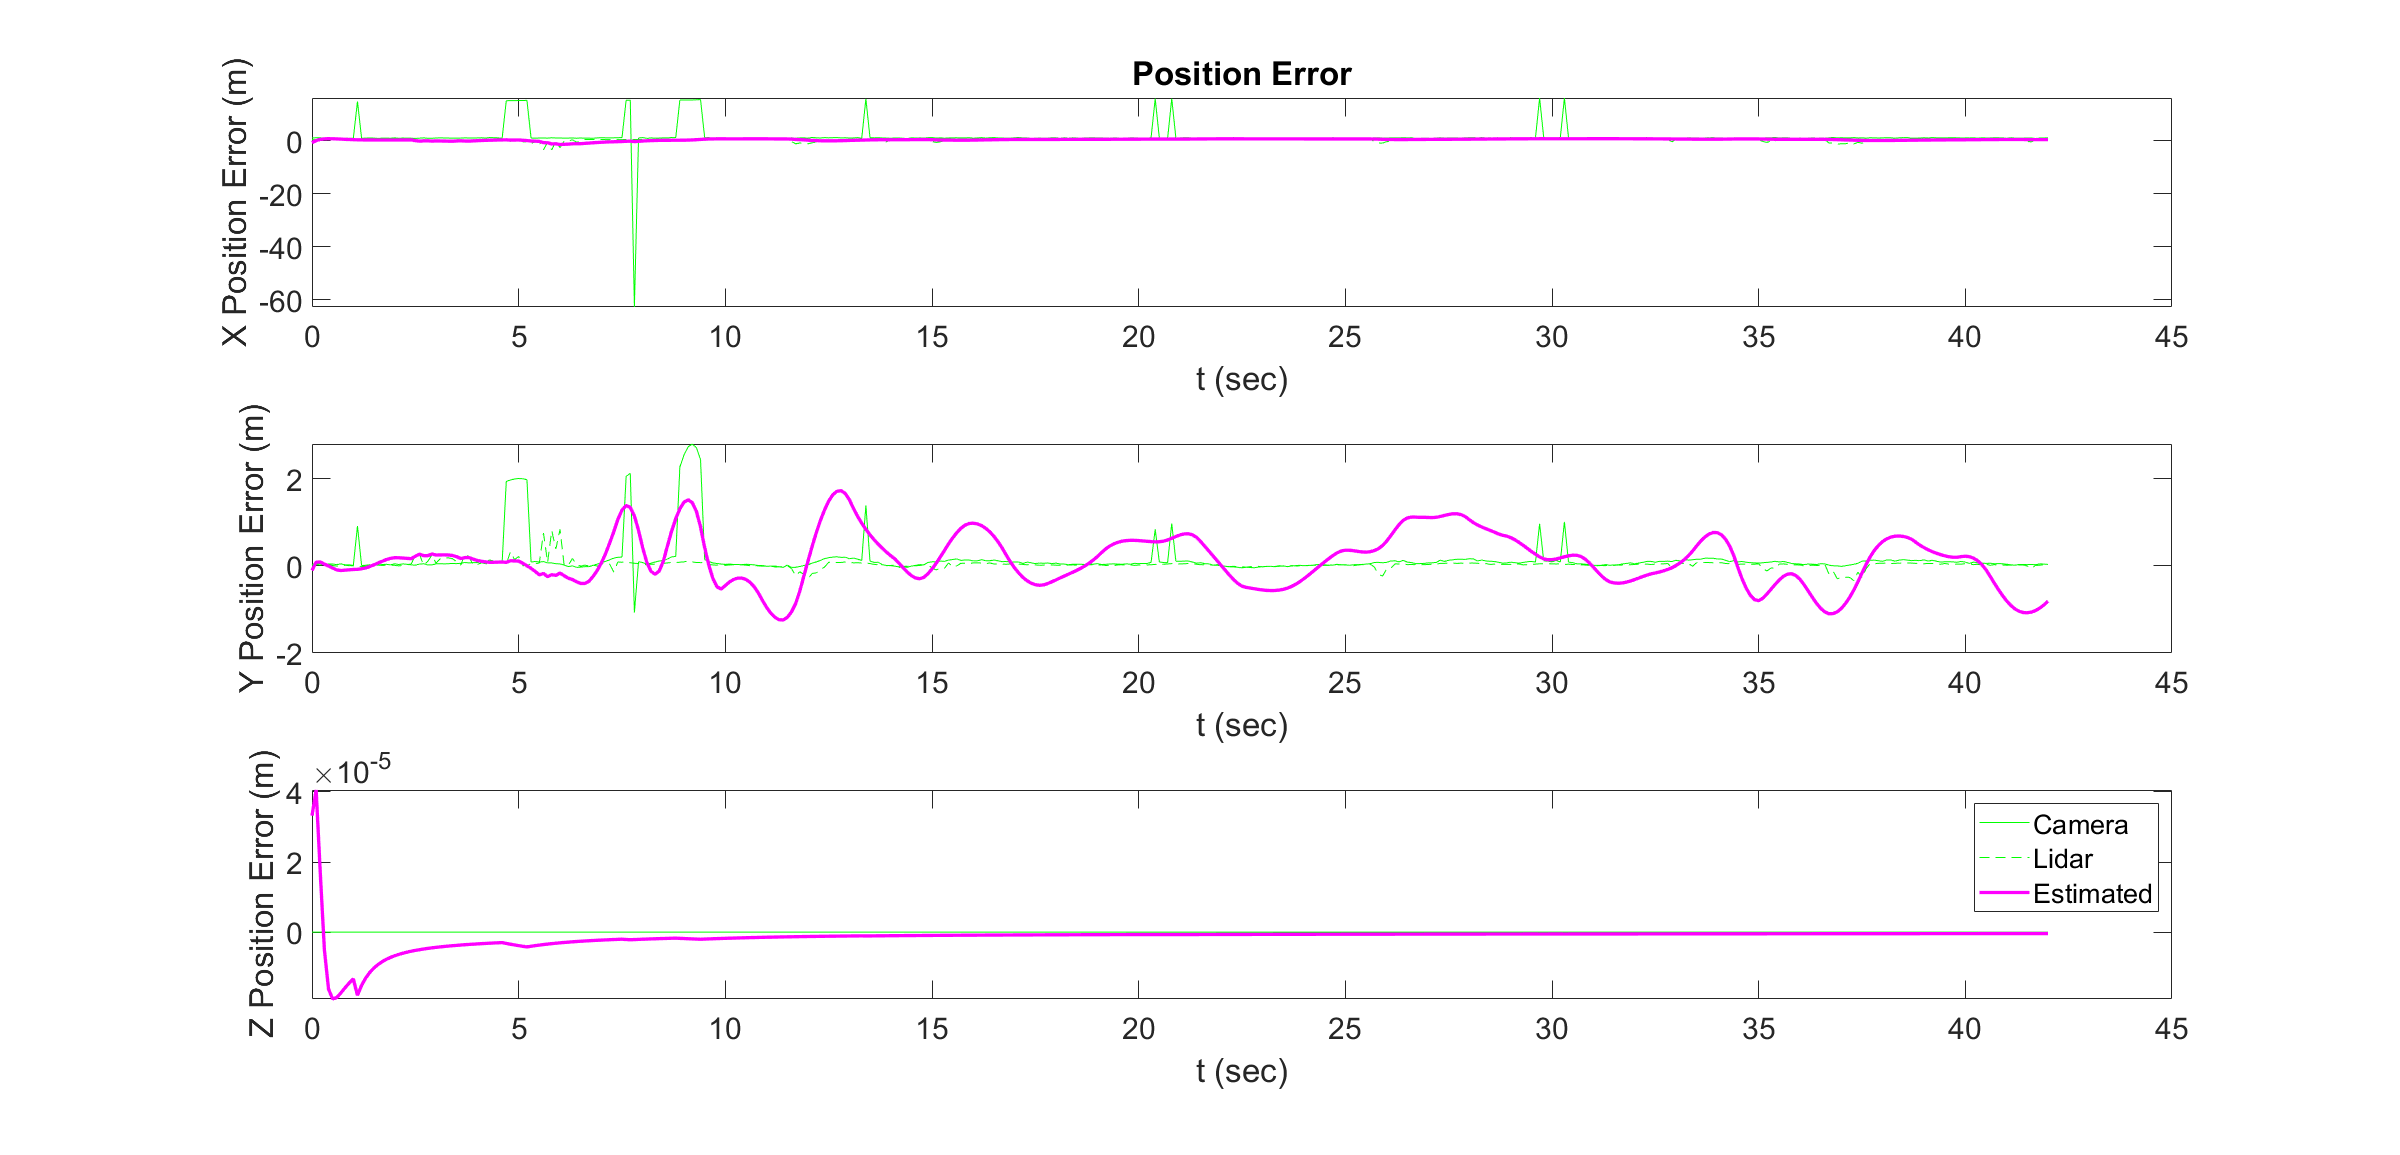
\includegraphics[width=1\textwidth]{Images/Residue_error_plot.png}
    \caption{Sensor Measurement and Estimation Error Plot}
\end{figure}
\end{frame}

%---------------------------------------------------------

%%%%%%Experimental Results%%%%%%%%%

\section{Experimental Results}

%---------------------------------------------------------
\begin{frame}{Co-ordinate Axis}
\begin{figure}
    \centering
    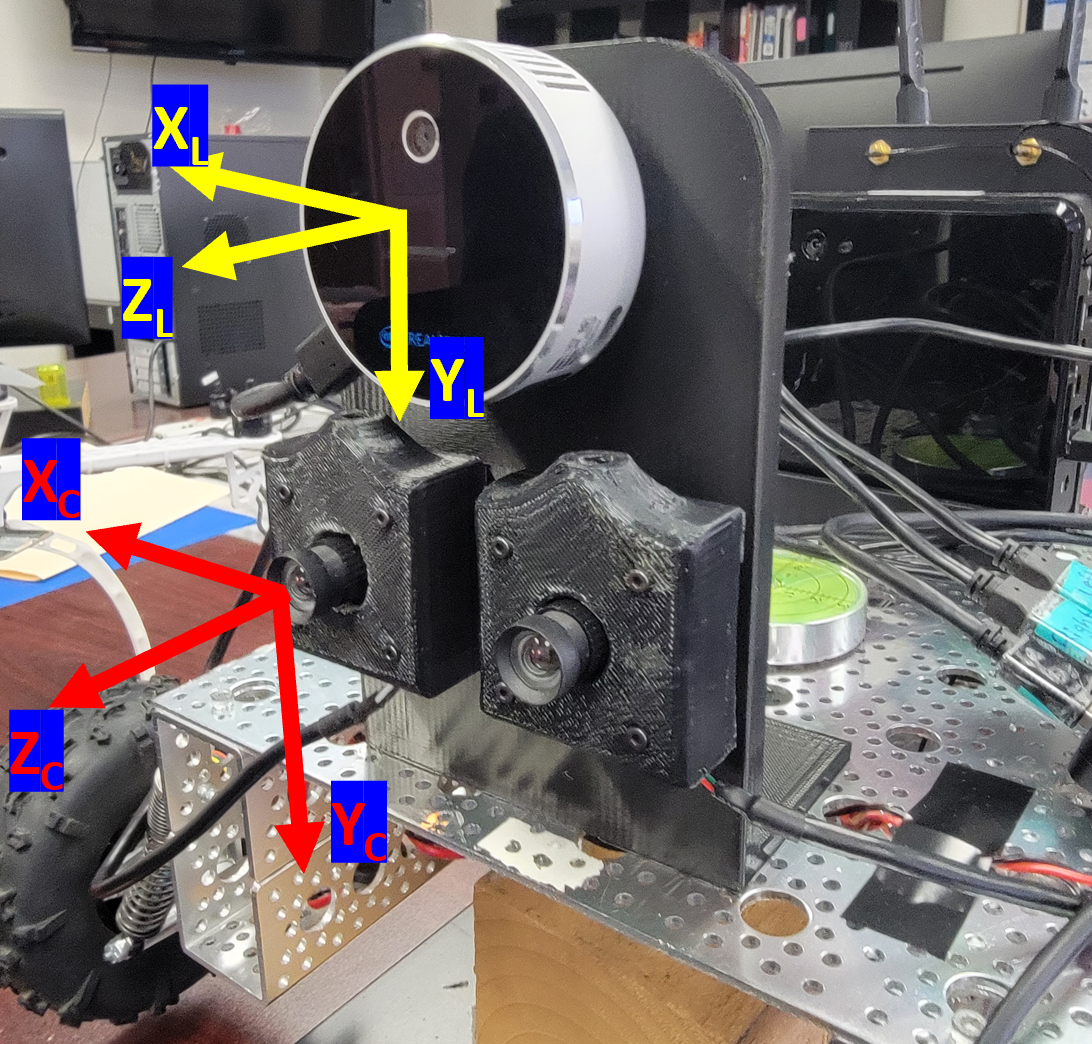
\includegraphics[width=0.5\textwidth]{Images/experimentalplateform.png}
\end{figure}
\end{frame}

\begin{frame}{Sensor Co-variance}
\large
\centering
$$R_{LiDAR} = 
    \left[\begin{array}{ccc}
    5.84e-05 & 0 & 0 \\
    0 & 2.73e-04 & 0 \\
    0 & 0 & 3.917e-06
    \end{array}\right]$$
    
$$  R_{Camera} =
    \left[\begin{array}{ccc}
    2.59e-05 & 0 & 0 \\
    0 & 9.76e-06 & 0 \\
    0 & 0 & 4.46e-04
    \end{array}\right]$$    
\end{frame}

\begin{frame}{Real-time Position Estimation}
\centering
 \huge
 Video
    
\end{frame}

\begin{frame}{Position Plot ''Box"}
\begin{figure}
    \centering
    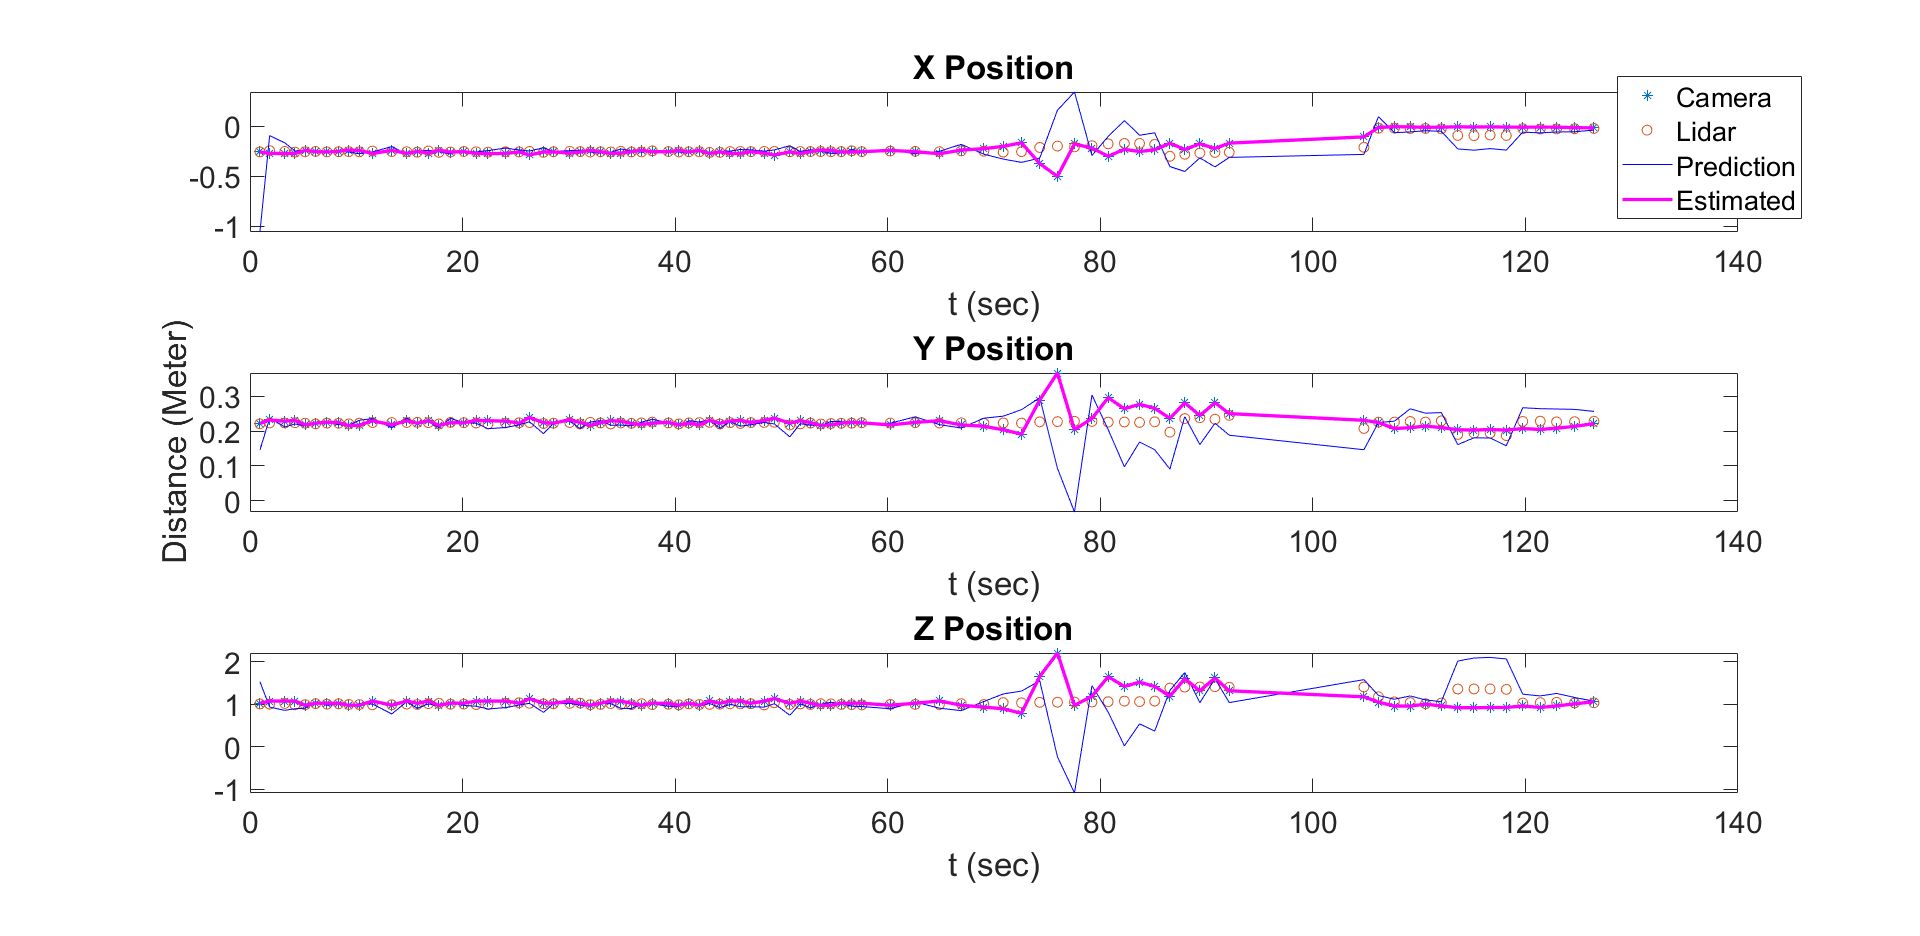
\includegraphics[width=1\textwidth]{Images/Box_position.png}
    \caption{Position plot of an Object ''Box"}
\end{figure}
\end{frame}

\begin{frame}{Velocity Plot ''Box"}
\begin{figure}
    \centering
    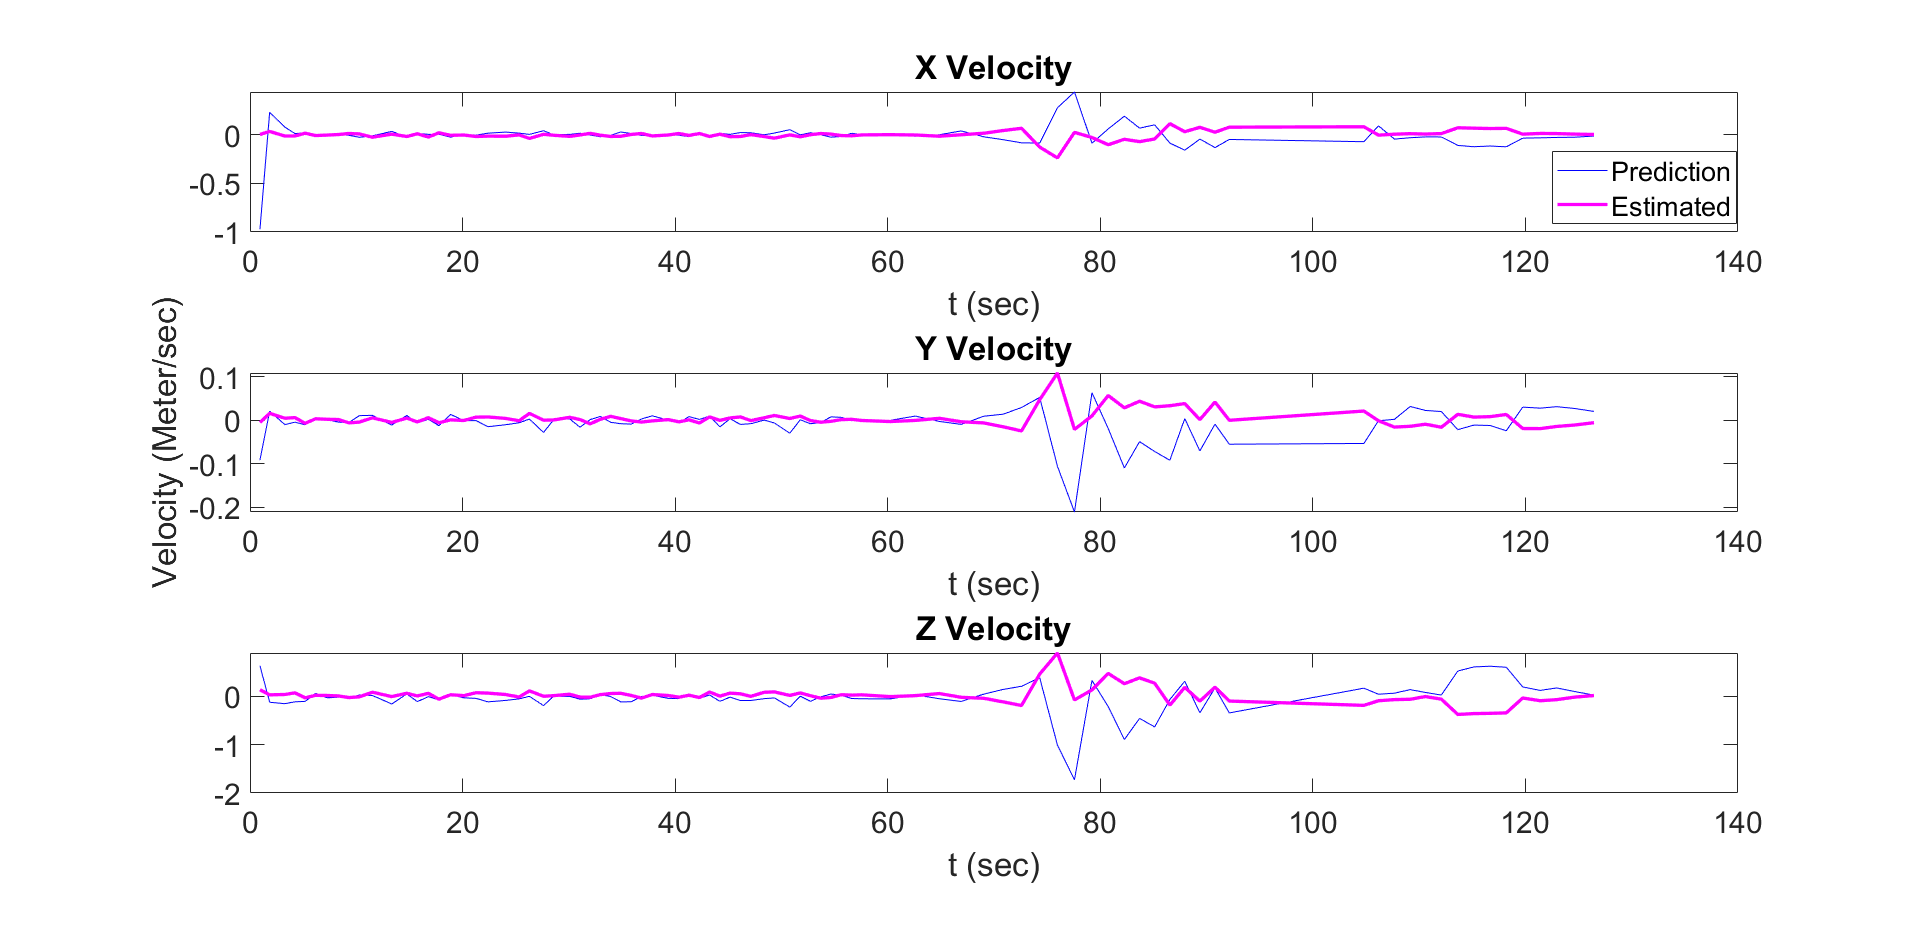
\includegraphics[width=1\textwidth]{Images/Box_velocity.png}
    \caption{Velocity plot of an Object ''Box"}
\end{figure}
\end{frame}

\begin{frame}{Position Plot ''Traffic Cone"}
\begin{figure}
    \centering
    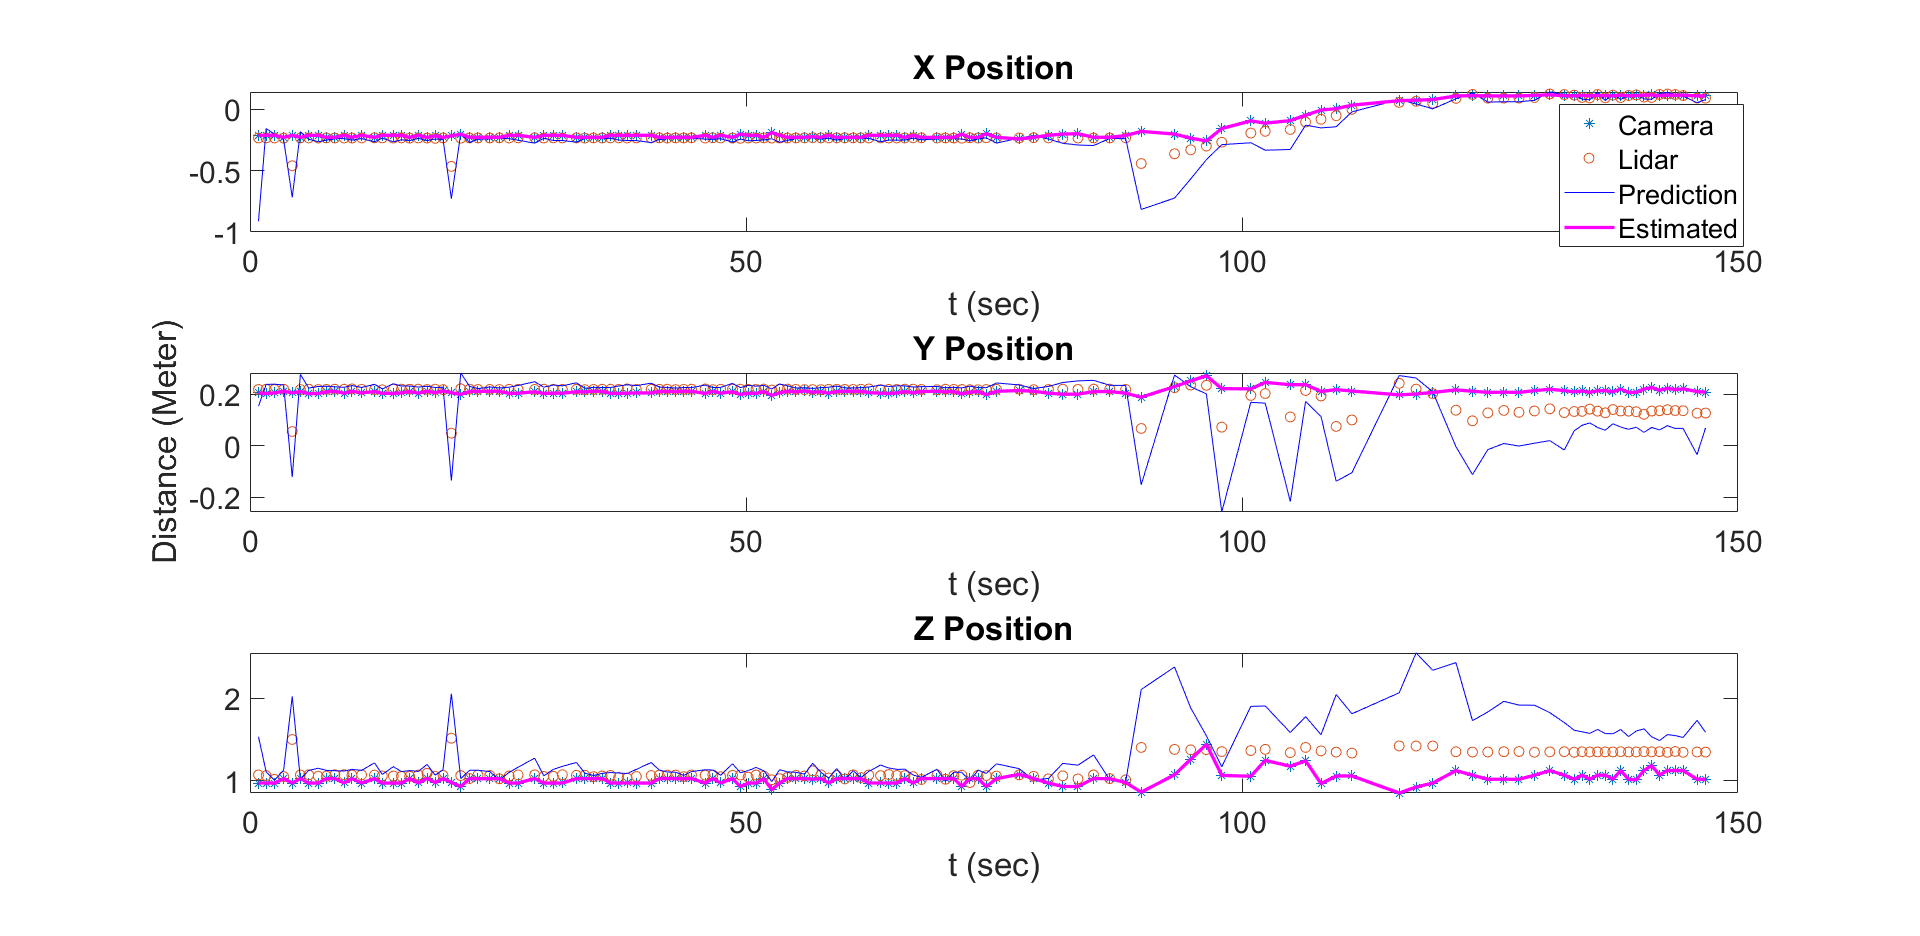
\includegraphics[width=1\textwidth]{Images/TC_position.png}
    \caption{Position plot of an Object ''Traffic Cone"}
\end{figure}
\end{frame}

\begin{frame}{Velocity Plot ''Traffic Cone"}
\begin{figure}
    \centering
    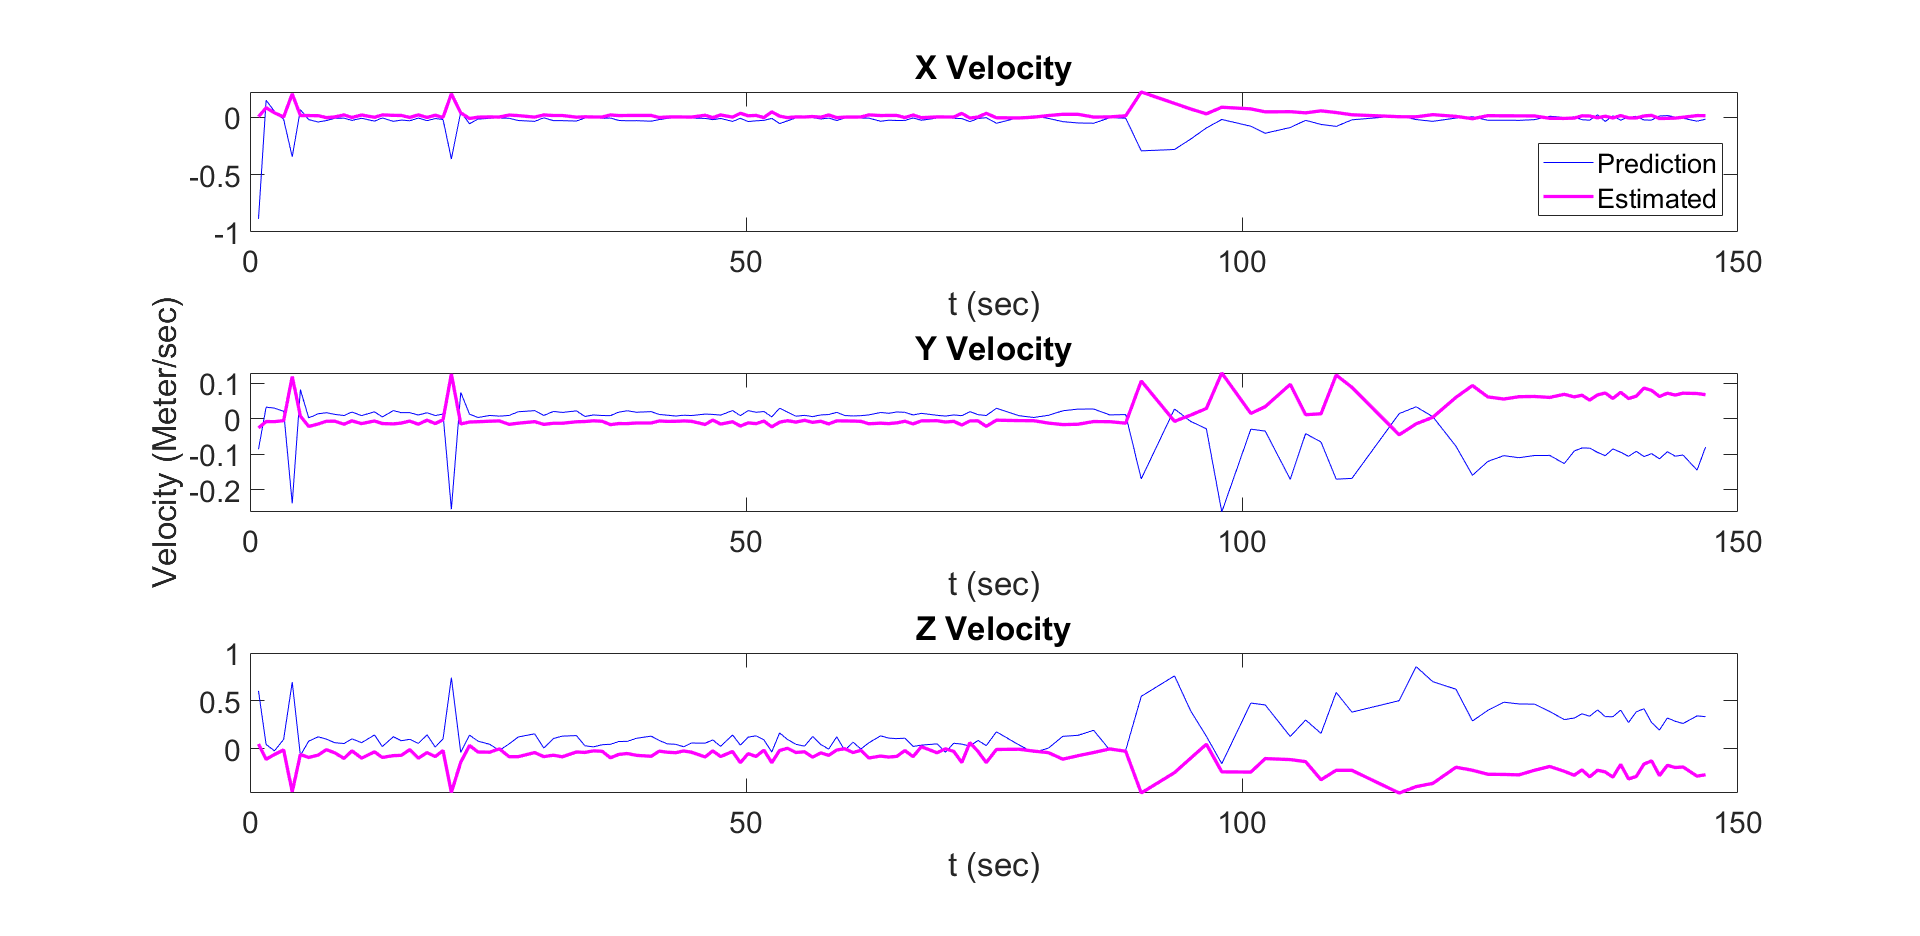
\includegraphics[width=1\textwidth]{Images/TC_velocity.png}
    \caption{Velocity plot of an Object ''Traffic Cone"}
\end{figure}
\end{frame}

%---------------------------------------------------------

%%%%%%Conclusion & Future Work%%%%%%%%%

\section{Conclusion \& Future Work}

%---------------------------------------------------------

\begin{frame}{Conclusion}
  \begin{itemize}
      \item It was shown in this work that the YOLO-v3 unified algorithm performs better and faster than most of the modern object detection neural networks.
      \item The training and testing accuracy of 99\% and 96\% respectively were achieved. 
      \item An intrinsic and extrinsic calibration of Lidar and stereo camera was carried out to compute the measurement and transformation error of camera and Lidar data.
      \item Finally, a sensor fusion algorithm was implemented by using a linear Kalman filter to fuse the data coming from Lidar and the stereo camera.
  \end{itemize}  
\end{frame}

\begin{frame}{Future Work}
\begin{itemize}
    \item Develop a more sophisticated multi-object tracking algorithm; for instance JPDA (Joint Probabilistic Data Association). 
    \item Further this study can be extended to implement the collision avoidance, and SLAM (Simultaneous Localization and Mapping).
    \item The neural network can be trained to detect more complex objects that might be encountered in the real world.
    \item The YOLO-v3 network is further tuned to improve test accuracy.
    \item By use of the LiDAR with a stronger laser that can use in ambient conditions, this research work can be extended to autonomous driving or advanced driving assistance system.
    \item The Lidar and camera calibrations can be automated and made more accurate to improve the overall system accuracy in the future. 
\end{itemize}    
\end{frame}


\end{document}